\documentclass[twoside]{book}

% Packages required by doxygen
\usepackage{fixltx2e}
\usepackage{calc}
\usepackage{doxygen}
\usepackage{graphicx}
\usepackage[utf8]{inputenc}
\usepackage{makeidx}
\usepackage{multicol}
\usepackage{multirow}
\PassOptionsToPackage{warn}{textcomp}
\usepackage{textcomp}
\usepackage[nointegrals]{wasysym}
\usepackage[table]{xcolor}

% Font selection
\usepackage[T1]{fontenc}
\usepackage{mathptmx}
\usepackage[scaled=.90]{helvet}
\usepackage{courier}
\usepackage{amssymb}
\usepackage{sectsty}
\renewcommand{\familydefault}{\sfdefault}
\allsectionsfont{%
  \fontseries{bc}\selectfont%
  \color{darkgray}%
}
\renewcommand{\DoxyLabelFont}{%
  \fontseries{bc}\selectfont%
  \color{darkgray}%
}
\newcommand{\+}{\discretionary{\mbox{\scriptsize$\hookleftarrow$}}{}{}}

% Page & text layout
\usepackage{geometry}
\geometry{%
  a4paper,%
  top=2.5cm,%
  bottom=2.5cm,%
  left=2.5cm,%
  right=2.5cm%
}
\tolerance=750
\hfuzz=15pt
\hbadness=750
\setlength{\emergencystretch}{15pt}
\setlength{\parindent}{0cm}
\setlength{\parskip}{0.2cm}
\makeatletter
\renewcommand{\paragraph}{%
  \@startsection{paragraph}{4}{0ex}{-1.0ex}{1.0ex}{%
    \normalfont\normalsize\bfseries\SS@parafont%
  }%
}
\renewcommand{\subparagraph}{%
  \@startsection{subparagraph}{5}{0ex}{-1.0ex}{1.0ex}{%
    \normalfont\normalsize\bfseries\SS@subparafont%
  }%
}
\makeatother

% Headers & footers
\usepackage{fancyhdr}
\pagestyle{fancyplain}
\fancyhead[LE]{\fancyplain{}{\bfseries\thepage}}
\fancyhead[CE]{\fancyplain{}{}}
\fancyhead[RE]{\fancyplain{}{\bfseries\leftmark}}
\fancyhead[LO]{\fancyplain{}{\bfseries\rightmark}}
\fancyhead[CO]{\fancyplain{}{}}
\fancyhead[RO]{\fancyplain{}{\bfseries\thepage}}
\fancyfoot[LE]{\fancyplain{}{}}
\fancyfoot[CE]{\fancyplain{}{}}
\fancyfoot[RE]{\fancyplain{}{\bfseries\scriptsize Generated on Mon Oct 19 2015 16\+:01\+:06 for T\+P3\+:\+Documentation du source by Doxygen }}
\fancyfoot[LO]{\fancyplain{}{\bfseries\scriptsize Generated on Mon Oct 19 2015 16\+:01\+:06 for T\+P3\+:\+Documentation du source by Doxygen }}
\fancyfoot[CO]{\fancyplain{}{}}
\fancyfoot[RO]{\fancyplain{}{}}
\renewcommand{\footrulewidth}{0.4pt}
\renewcommand{\chaptermark}[1]{%
  \markboth{#1}{}%
}
\renewcommand{\sectionmark}[1]{%
  \markright{\thesection\ #1}%
}

% Indices & bibliography
\usepackage{natbib}
\usepackage[titles]{tocloft}
\setcounter{tocdepth}{3}
\setcounter{secnumdepth}{5}
\makeindex

% Hyperlinks (required, but should be loaded last)
\usepackage{ifpdf}
\ifpdf
  \usepackage[pdftex,pagebackref=true]{hyperref}
\else
  \usepackage[ps2pdf,pagebackref=true]{hyperref}
\fi
\hypersetup{%
  colorlinks=true,%
  linkcolor=blue,%
  citecolor=blue,%
  unicode%
}

% Custom commands
\newcommand{\clearemptydoublepage}{%
  \newpage{\pagestyle{empty}\cleardoublepage}%
}


%===== C O N T E N T S =====

\begin{document}

% Titlepage & ToC
\hypersetup{pageanchor=false,
             bookmarks=true,
             bookmarksnumbered=true,
             pdfencoding=unicode
            }
\pagenumbering{roman}
\begin{titlepage}
\vspace*{7cm}
\begin{center}%
{\Large T\+P3\+:Documentation du source \\[1ex]\large 1.\+0 }\\
\vspace*{1cm}
{\large Generated by Doxygen 1.8.7}\\
\vspace*{0.5cm}
{\small Mon Oct 19 2015 16:01:06}\\
\end{center}
\end{titlepage}
\clearemptydoublepage
\tableofcontents
\clearemptydoublepage
\pagenumbering{arabic}
\hypersetup{pageanchor=true}

%--- Begin generated contents ---
\chapter{Data Structure Index}
\section{Data Structures}
Here are the data structures with brief descriptions\+:\begin{DoxyCompactList}
\item\contentsline{section}{\hyperlink{classPDFlib_1_1Exception}{P\+D\+Flib\+::\+Exception} }{\pageref{classPDFlib_1_1Exception}}{}
\item\contentsline{section}{\hyperlink{classFonctions}{Fonctions} \\*Classe intanciant un pdflib nous permettant d'executer des manipulations sur le pdf }{\pageref{classFonctions}}{}
\item\contentsline{section}{\hyperlink{classPDFlib}{P\+D\+Flib} }{\pageref{classPDFlib}}{}
\end{DoxyCompactList}

\chapter{File Index}
\section{File List}
Here is a list of all files with brief descriptions\+:\begin{DoxyCompactList}
\item\contentsline{section}{\hyperlink{Fonctions_8cpp}{Fonctions.\+cpp} }{\pageref{Fonctions_8cpp}}{}
\item\contentsline{section}{\hyperlink{Fonctions_8hpp}{Fonctions.\+hpp} \\*\hyperlink{classFonctions}{Fonctions} permettant de générer des graphes au format pdf }{\pageref{Fonctions_8hpp}}{}
\item\contentsline{section}{\hyperlink{main_8cpp}{main.\+cpp} }{\pageref{main_8cpp}}{}
\item\contentsline{section}{\hyperlink{pdflib_8cpp}{pdflib.\+cpp} }{\pageref{pdflib_8cpp}}{}
\item\contentsline{section}{\hyperlink{pdflib_8hpp}{pdflib.\+hpp} }{\pageref{pdflib_8hpp}}{}
\end{DoxyCompactList}

\chapter{Data Structure Documentation}
\hypertarget{classPDFlib_1_1Exception}{\section{P\+D\+Flib\+:\+:Exception Class Reference}
\label{classPDFlib_1_1Exception}\index{P\+D\+Flib\+::\+Exception@{P\+D\+Flib\+::\+Exception}}
}


{\ttfamily \#include $<$pdflib.\+hpp$>$}



Collaboration diagram for P\+D\+Flib\+:\+:Exception\+:\nopagebreak
\begin{figure}[H]
\begin{center}
\leavevmode
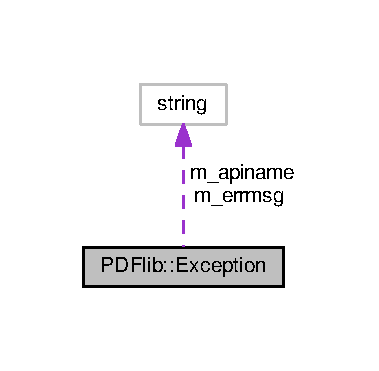
\includegraphics[width=182pt]{classPDFlib_1_1Exception__coll__graph}
\end{center}
\end{figure}
\subsection*{Public Member Functions}
\begin{DoxyCompactItemize}
\item 
\hyperlink{classPDFlib_1_1Exception_a57fa9533e1498e00612ac13349c78ac8}{Exception} (std\+::string errmsg, int errnum, std\+::string apiname, void $\ast$opaque)
\item 
std\+::string \hyperlink{classPDFlib_1_1Exception_a0a197e182bf824c5654f721bf18debbf}{get\+\_\+errmsg} ()
\item 
int \hyperlink{classPDFlib_1_1Exception_aa29ae977a69d26d5a6aea1da399ff599}{get\+\_\+errnum} ()
\item 
std\+::string \hyperlink{classPDFlib_1_1Exception_a1463d47b0cb8d9f2251ffcbede9f6310}{get\+\_\+apiname} ()
\item 
const void $\ast$ \hyperlink{classPDFlib_1_1Exception_a6a286472fd0e02d9a02d24c2d83478f1}{get\+\_\+opaque} ()
\end{DoxyCompactItemize}
\subsection*{Private Attributes}
\begin{DoxyCompactItemize}
\item 
std\+::string \hyperlink{classPDFlib_1_1Exception_a03c21a477c8645b05e3f4b8367f14d47}{m\+\_\+errmsg}
\item 
int \hyperlink{classPDFlib_1_1Exception_a768df1c2eeb409c9d5a5814bc2d367dc}{m\+\_\+errnum}
\item 
std\+::string \hyperlink{classPDFlib_1_1Exception_a23e1637eebbe959aa47c80c81f0fd386}{m\+\_\+apiname}
\item 
void $\ast$ \hyperlink{classPDFlib_1_1Exception_ab18c530da60097292993918457fa0171}{m\+\_\+opaque}
\end{DoxyCompactItemize}


\subsection{Constructor \& Destructor Documentation}
\hypertarget{classPDFlib_1_1Exception_a57fa9533e1498e00612ac13349c78ac8}{\index{P\+D\+Flib\+::\+Exception@{P\+D\+Flib\+::\+Exception}!Exception@{Exception}}
\index{Exception@{Exception}!P\+D\+Flib\+::\+Exception@{P\+D\+Flib\+::\+Exception}}
\subsubsection[{Exception}]{\setlength{\rightskip}{0pt plus 5cm}P\+D\+Flib\+::\+Exception\+::\+Exception (
\begin{DoxyParamCaption}
\item[{std\+::string}]{errmsg, }
\item[{int}]{errnum, }
\item[{std\+::string}]{apiname, }
\item[{void $\ast$}]{opaque}
\end{DoxyParamCaption}
)}}\label{classPDFlib_1_1Exception_a57fa9533e1498e00612ac13349c78ac8}


\subsection{Member Function Documentation}
\hypertarget{classPDFlib_1_1Exception_a1463d47b0cb8d9f2251ffcbede9f6310}{\index{P\+D\+Flib\+::\+Exception@{P\+D\+Flib\+::\+Exception}!get\+\_\+apiname@{get\+\_\+apiname}}
\index{get\+\_\+apiname@{get\+\_\+apiname}!P\+D\+Flib\+::\+Exception@{P\+D\+Flib\+::\+Exception}}
\subsubsection[{get\+\_\+apiname}]{\setlength{\rightskip}{0pt plus 5cm}string P\+D\+Flib\+::\+Exception\+::get\+\_\+apiname (
\begin{DoxyParamCaption}
{}
\end{DoxyParamCaption}
)}}\label{classPDFlib_1_1Exception_a1463d47b0cb8d9f2251ffcbede9f6310}
\hypertarget{classPDFlib_1_1Exception_a0a197e182bf824c5654f721bf18debbf}{\index{P\+D\+Flib\+::\+Exception@{P\+D\+Flib\+::\+Exception}!get\+\_\+errmsg@{get\+\_\+errmsg}}
\index{get\+\_\+errmsg@{get\+\_\+errmsg}!P\+D\+Flib\+::\+Exception@{P\+D\+Flib\+::\+Exception}}
\subsubsection[{get\+\_\+errmsg}]{\setlength{\rightskip}{0pt plus 5cm}string P\+D\+Flib\+::\+Exception\+::get\+\_\+errmsg (
\begin{DoxyParamCaption}
{}
\end{DoxyParamCaption}
)}}\label{classPDFlib_1_1Exception_a0a197e182bf824c5654f721bf18debbf}
\hypertarget{classPDFlib_1_1Exception_aa29ae977a69d26d5a6aea1da399ff599}{\index{P\+D\+Flib\+::\+Exception@{P\+D\+Flib\+::\+Exception}!get\+\_\+errnum@{get\+\_\+errnum}}
\index{get\+\_\+errnum@{get\+\_\+errnum}!P\+D\+Flib\+::\+Exception@{P\+D\+Flib\+::\+Exception}}
\subsubsection[{get\+\_\+errnum}]{\setlength{\rightskip}{0pt plus 5cm}int P\+D\+Flib\+::\+Exception\+::get\+\_\+errnum (
\begin{DoxyParamCaption}
{}
\end{DoxyParamCaption}
)}}\label{classPDFlib_1_1Exception_aa29ae977a69d26d5a6aea1da399ff599}
\hypertarget{classPDFlib_1_1Exception_a6a286472fd0e02d9a02d24c2d83478f1}{\index{P\+D\+Flib\+::\+Exception@{P\+D\+Flib\+::\+Exception}!get\+\_\+opaque@{get\+\_\+opaque}}
\index{get\+\_\+opaque@{get\+\_\+opaque}!P\+D\+Flib\+::\+Exception@{P\+D\+Flib\+::\+Exception}}
\subsubsection[{get\+\_\+opaque}]{\setlength{\rightskip}{0pt plus 5cm}const void $\ast$ P\+D\+Flib\+::\+Exception\+::get\+\_\+opaque (
\begin{DoxyParamCaption}
{}
\end{DoxyParamCaption}
)}}\label{classPDFlib_1_1Exception_a6a286472fd0e02d9a02d24c2d83478f1}


\subsection{Field Documentation}
\hypertarget{classPDFlib_1_1Exception_a23e1637eebbe959aa47c80c81f0fd386}{\index{P\+D\+Flib\+::\+Exception@{P\+D\+Flib\+::\+Exception}!m\+\_\+apiname@{m\+\_\+apiname}}
\index{m\+\_\+apiname@{m\+\_\+apiname}!P\+D\+Flib\+::\+Exception@{P\+D\+Flib\+::\+Exception}}
\subsubsection[{m\+\_\+apiname}]{\setlength{\rightskip}{0pt plus 5cm}std\+::string P\+D\+Flib\+::\+Exception\+::m\+\_\+apiname\hspace{0.3cm}{\ttfamily [private]}}}\label{classPDFlib_1_1Exception_a23e1637eebbe959aa47c80c81f0fd386}
\hypertarget{classPDFlib_1_1Exception_a03c21a477c8645b05e3f4b8367f14d47}{\index{P\+D\+Flib\+::\+Exception@{P\+D\+Flib\+::\+Exception}!m\+\_\+errmsg@{m\+\_\+errmsg}}
\index{m\+\_\+errmsg@{m\+\_\+errmsg}!P\+D\+Flib\+::\+Exception@{P\+D\+Flib\+::\+Exception}}
\subsubsection[{m\+\_\+errmsg}]{\setlength{\rightskip}{0pt plus 5cm}std\+::string P\+D\+Flib\+::\+Exception\+::m\+\_\+errmsg\hspace{0.3cm}{\ttfamily [private]}}}\label{classPDFlib_1_1Exception_a03c21a477c8645b05e3f4b8367f14d47}
\hypertarget{classPDFlib_1_1Exception_a768df1c2eeb409c9d5a5814bc2d367dc}{\index{P\+D\+Flib\+::\+Exception@{P\+D\+Flib\+::\+Exception}!m\+\_\+errnum@{m\+\_\+errnum}}
\index{m\+\_\+errnum@{m\+\_\+errnum}!P\+D\+Flib\+::\+Exception@{P\+D\+Flib\+::\+Exception}}
\subsubsection[{m\+\_\+errnum}]{\setlength{\rightskip}{0pt plus 5cm}int P\+D\+Flib\+::\+Exception\+::m\+\_\+errnum\hspace{0.3cm}{\ttfamily [private]}}}\label{classPDFlib_1_1Exception_a768df1c2eeb409c9d5a5814bc2d367dc}
\hypertarget{classPDFlib_1_1Exception_ab18c530da60097292993918457fa0171}{\index{P\+D\+Flib\+::\+Exception@{P\+D\+Flib\+::\+Exception}!m\+\_\+opaque@{m\+\_\+opaque}}
\index{m\+\_\+opaque@{m\+\_\+opaque}!P\+D\+Flib\+::\+Exception@{P\+D\+Flib\+::\+Exception}}
\subsubsection[{m\+\_\+opaque}]{\setlength{\rightskip}{0pt plus 5cm}void$\ast$ P\+D\+Flib\+::\+Exception\+::m\+\_\+opaque\hspace{0.3cm}{\ttfamily [private]}}}\label{classPDFlib_1_1Exception_ab18c530da60097292993918457fa0171}


The documentation for this class was generated from the following files\+:\begin{DoxyCompactItemize}
\item 
\hyperlink{pdflib_8hpp}{pdflib.\+hpp}\item 
\hyperlink{pdflib_8cpp}{pdflib.\+cpp}\end{DoxyCompactItemize}

\hypertarget{classFonctions}{\section{Fonctions Class Reference}
\label{classFonctions}\index{Fonctions@{Fonctions}}
}


classe intanciant un pdflib nous permettant d'executer des manipulations sur le pdf.  




{\ttfamily \#include $<$Fonctions.\+hpp$>$}



Collaboration diagram for Fonctions\+:\nopagebreak
\begin{figure}[H]
\begin{center}
\leavevmode
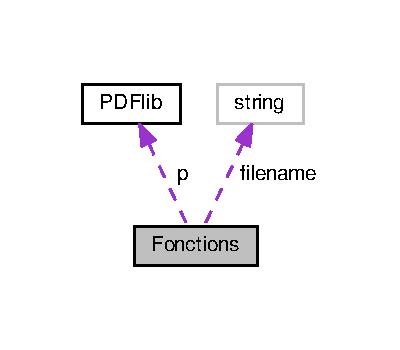
\includegraphics[width=192pt]{classFonctions__coll__graph}
\end{center}
\end{figure}
\subsection*{Public Member Functions}
\begin{DoxyCompactItemize}
\item 
\hyperlink{classFonctions_a3def9621d78c611beb962e4a73829e8f}{Fonctions} ()
\item 
void \hyperlink{classFonctions_a5539501c7d6cb67f829e8f578197e23f}{make\+A4} ()
\begin{DoxyCompactList}\small\item\em Génère une feuille A4 vierge au format P\+D\+F. \end{DoxyCompactList}\item 
void \hyperlink{classFonctions_a56328671ad685e595b7d0c1a4d7ff233}{end\+Doc} ()
\begin{DoxyCompactList}\small\item\em Cette fonction doit etre appelée obligatoirement. Elle sert a terminer le Document pdf. Sans celle-\/ci votre document ne fonctionnera pas. \end{DoxyCompactList}\item 
void \hyperlink{classFonctions_aa8d950f493acc58fd3e48730559b4ac5}{essai\+Cercle} ()
\begin{DoxyCompactList}\small\item\em fait un petit dessin test de cercle au centre du pdf. \end{DoxyCompactList}\item 
void \hyperlink{classFonctions_ad4e849db3ce1595c7a8bb2eb746b09d5}{ask\+Filename} ()
\begin{DoxyCompactList}\small\item\em Demande à l'utilisateur une chaine de caractère. Cette chaine doit représenter le nom du fichier à lire. Modifie l'attribut filename. \end{DoxyCompactList}\item 
\hyperlink{classFonctions_a6d7062796a65e0e15f3b3aa3cfacd08f}{$\sim$\+Fonctions} ()
\end{DoxyCompactItemize}
\subsection*{Private Attributes}
\begin{DoxyCompactItemize}
\item 
\hyperlink{classPDFlib}{P\+D\+Flib} $\ast$ \hyperlink{classFonctions_a6ade569c9a4303f29d50f2ac4c771977}{p}
\item 
Text\+Manager $\ast$ \hyperlink{classFonctions_aa425e8c464cd5dda67be23a405b71135}{tm}
\begin{DoxyCompactList}\small\item\em utilisé pour creer les pdfs \end{DoxyCompactList}\item 
std\+::string \hyperlink{classFonctions_a08652f255d6c1ddfc018c8796f38c606}{filename}
\begin{DoxyCompactList}\small\item\em utilisé pour lire les fichiers de données \end{DoxyCompactList}\end{DoxyCompactItemize}


\subsection{Detailed Description}
classe intanciant un pdflib nous permettant d'executer des manipulations sur le pdf. 

\subsection{Constructor \& Destructor Documentation}
\hypertarget{classFonctions_a3def9621d78c611beb962e4a73829e8f}{\index{Fonctions@{Fonctions}!Fonctions@{Fonctions}}
\index{Fonctions@{Fonctions}!Fonctions@{Fonctions}}
\subsubsection[{Fonctions}]{\setlength{\rightskip}{0pt plus 5cm}Fonctions\+::\+Fonctions (
\begin{DoxyParamCaption}
{}
\end{DoxyParamCaption}
)}}\label{classFonctions_a3def9621d78c611beb962e4a73829e8f}
\hypertarget{classFonctions_a6d7062796a65e0e15f3b3aa3cfacd08f}{\index{Fonctions@{Fonctions}!````~Fonctions@{$\sim$\+Fonctions}}
\index{````~Fonctions@{$\sim$\+Fonctions}!Fonctions@{Fonctions}}
\subsubsection[{$\sim$\+Fonctions}]{\setlength{\rightskip}{0pt plus 5cm}Fonctions\+::$\sim$\+Fonctions (
\begin{DoxyParamCaption}
{}
\end{DoxyParamCaption}
)}}\label{classFonctions_a6d7062796a65e0e15f3b3aa3cfacd08f}


\subsection{Member Function Documentation}
\hypertarget{classFonctions_ad4e849db3ce1595c7a8bb2eb746b09d5}{\index{Fonctions@{Fonctions}!ask\+Filename@{ask\+Filename}}
\index{ask\+Filename@{ask\+Filename}!Fonctions@{Fonctions}}
\subsubsection[{ask\+Filename}]{\setlength{\rightskip}{0pt plus 5cm}void Fonctions\+::ask\+Filename (
\begin{DoxyParamCaption}
{}
\end{DoxyParamCaption}
)}}\label{classFonctions_ad4e849db3ce1595c7a8bb2eb746b09d5}


Demande à l'utilisateur une chaine de caractère. Cette chaine doit représenter le nom du fichier à lire. Modifie l'attribut filename. 

\hypertarget{classFonctions_a56328671ad685e595b7d0c1a4d7ff233}{\index{Fonctions@{Fonctions}!end\+Doc@{end\+Doc}}
\index{end\+Doc@{end\+Doc}!Fonctions@{Fonctions}}
\subsubsection[{end\+Doc}]{\setlength{\rightskip}{0pt plus 5cm}void Fonctions\+::end\+Doc (
\begin{DoxyParamCaption}
{}
\end{DoxyParamCaption}
)}}\label{classFonctions_a56328671ad685e595b7d0c1a4d7ff233}


Cette fonction doit etre appelée obligatoirement. Elle sert a terminer le Document pdf. Sans celle-\/ci votre document ne fonctionnera pas. 

\hypertarget{classFonctions_aa8d950f493acc58fd3e48730559b4ac5}{\index{Fonctions@{Fonctions}!essai\+Cercle@{essai\+Cercle}}
\index{essai\+Cercle@{essai\+Cercle}!Fonctions@{Fonctions}}
\subsubsection[{essai\+Cercle}]{\setlength{\rightskip}{0pt plus 5cm}void Fonctions\+::essai\+Cercle (
\begin{DoxyParamCaption}
{}
\end{DoxyParamCaption}
)}}\label{classFonctions_aa8d950f493acc58fd3e48730559b4ac5}


fait un petit dessin test de cercle au centre du pdf. 

\hypertarget{classFonctions_a5539501c7d6cb67f829e8f578197e23f}{\index{Fonctions@{Fonctions}!make\+A4@{make\+A4}}
\index{make\+A4@{make\+A4}!Fonctions@{Fonctions}}
\subsubsection[{make\+A4}]{\setlength{\rightskip}{0pt plus 5cm}void Fonctions\+::make\+A4 (
\begin{DoxyParamCaption}
{}
\end{DoxyParamCaption}
)}}\label{classFonctions_a5539501c7d6cb67f829e8f578197e23f}


Génère une feuille A4 vierge au format P\+D\+F. 

\begin{DoxyWarning}{Warning}
Attention \+: n'oubliez pas d'appeler \hyperlink{classFonctions_a56328671ad685e595b7d0c1a4d7ff233}{end\+Doc()} afin de terminer votre fichier. 
\end{DoxyWarning}


\subsection{Field Documentation}
\hypertarget{classFonctions_a08652f255d6c1ddfc018c8796f38c606}{\index{Fonctions@{Fonctions}!filename@{filename}}
\index{filename@{filename}!Fonctions@{Fonctions}}
\subsubsection[{filename}]{\setlength{\rightskip}{0pt plus 5cm}std\+::string Fonctions\+::filename\hspace{0.3cm}{\ttfamily [private]}}}\label{classFonctions_a08652f255d6c1ddfc018c8796f38c606}


utilisé pour lire les fichiers de données 

\hypertarget{classFonctions_a6ade569c9a4303f29d50f2ac4c771977}{\index{Fonctions@{Fonctions}!p@{p}}
\index{p@{p}!Fonctions@{Fonctions}}
\subsubsection[{p}]{\setlength{\rightskip}{0pt plus 5cm}{\bf P\+D\+Flib}$\ast$ Fonctions\+::p\hspace{0.3cm}{\ttfamily [private]}}}\label{classFonctions_a6ade569c9a4303f29d50f2ac4c771977}
\hypertarget{classFonctions_aa425e8c464cd5dda67be23a405b71135}{\index{Fonctions@{Fonctions}!tm@{tm}}
\index{tm@{tm}!Fonctions@{Fonctions}}
\subsubsection[{tm}]{\setlength{\rightskip}{0pt plus 5cm}Text\+Manager$\ast$ Fonctions\+::tm\hspace{0.3cm}{\ttfamily [private]}}}\label{classFonctions_aa425e8c464cd5dda67be23a405b71135}


utilisé pour creer les pdfs 



The documentation for this class was generated from the following files\+:\begin{DoxyCompactItemize}
\item 
\hyperlink{Fonctions_8hpp}{Fonctions.\+hpp}\item 
\hyperlink{Fonctions_8cpp}{Fonctions.\+cpp}\end{DoxyCompactItemize}

\hypertarget{classPDFlib}{\section{P\+D\+Flib Class Reference}
\label{classPDFlib}\index{P\+D\+Flib@{P\+D\+Flib}}
}


{\ttfamily \#include $<$pdflib.\+hpp$>$}

\subsection*{Data Structures}
\begin{DoxyCompactItemize}
\item 
class \hyperlink{classPDFlib_1_1Exception}{Exception}
\end{DoxyCompactItemize}
\subsection*{Public Member Functions}
\begin{DoxyCompactItemize}
\item 
\hyperlink{classPDFlib_a63a60e9b1c4c18e6db742f85011510f3}{P\+D\+Flib} (allocproc\+\_\+t allocproc=N\+U\+L\+L, reallocproc\+\_\+t reallocproc=N\+U\+L\+L, freeproc\+\_\+t freeproc=N\+U\+L\+L, void $\ast$opaque=N\+U\+L\+L)
\item 
\hyperlink{classPDFlib_aac6122db0d8f9eaaf26862f88d2f33ef}{$\sim$\+P\+D\+Flib} ()  throw ()
\item 
void \hyperlink{classPDFlib_a83cf7a11d217af0e33e6dca6267965c4}{activate\+\_\+item} (int id)
\item 
int \hyperlink{classPDFlib_afbf7e219b67e0099610963c1ca9b6dca}{add\+\_\+bookmark} (std\+::string text, int parent, int p\+\_\+open)
\item 
void \hyperlink{classPDFlib_a32faa0f4597b6dceacd54a4a5497823d}{add\+\_\+launchlink} (double llx, double lly, double urx, double ury, std\+::string filename)
\item 
void \hyperlink{classPDFlib_a2d47dcbd27a69e9c1c02ca608f927ab7}{add\+\_\+locallink} (double llx, double lly, double urx, double ury, int page, std\+::string optlist)
\item 
void \hyperlink{classPDFlib_a16845662dabe0494d69b016846f2adcc}{add\+\_\+nameddest} (std\+::string name, std\+::string optlist)
\item 
void \hyperlink{classPDFlib_ab054c136755f297058ac9812adefafec}{add\+\_\+note} (double llx, double lly, double urx, double ury, std\+::string contents, std\+::string title, std\+::string icon, int p\+\_\+open)
\item 
void \hyperlink{classPDFlib_acc2002bc0e060620bfe97eae7dcc9371}{add\+\_\+pdflink} (double llx, double lly, double urx, double ury, std\+::string filename, int page, std\+::string optlist)
\item 
int \hyperlink{classPDFlib_a153ce04a9c160a24d13763f8ba6578fa}{add\+\_\+table\+\_\+cell} (int table, int column, int row, std\+::string text, std\+::string optlist)
\item 
int \hyperlink{classPDFlib_a44f52fd96b6152a2b4ae4f71cebcf36b}{add\+\_\+textflow} (int textflow, std\+::string text, std\+::string optlist)
\item 
void \hyperlink{classPDFlib_a7561fadef64e392f98d047d5b6e79946}{add\+\_\+thumbnail} (int image)
\item 
void \hyperlink{classPDFlib_afdba46325698218399dda4b415204edd}{add\+\_\+weblink} (double llx, double lly, double urx, double ury, std\+::string url)
\item 
void \hyperlink{classPDFlib_aee884c54b243c01230926f493f06eaf9}{arc} (double x, double y, double r, double alpha, double beta)
\item 
void \hyperlink{classPDFlib_a061eb6bb4e041c52547cf9d58416ddac}{arcn} (double x, double y, double r, double alpha, double beta)
\item 
void \hyperlink{classPDFlib_a911b3c91d2670200cdb3b78742fc6980}{attach\+\_\+file} (double llx, double lly, double urx, double ury, std\+::string filename, std\+::string description, std\+::string author, std\+::string mimetype, std\+::string icon)
\item 
int \hyperlink{classPDFlib_aacb38db7f6eada3409fb616bd823e79f}{begin\+\_\+document} (std\+::string filename, std\+::string optlist)
\item 
void \hyperlink{classPDFlib_a0c3289b502ca325c222c4df9c8318d1f}{begin\+\_\+document\+\_\+callback} (writeproc\+\_\+t writeproc, std\+::string optlist)
\item 
void \hyperlink{classPDFlib_a3f8a5ee80b6c632c1687e3100ef4a1bb}{begin\+\_\+font} (std\+::string fontname, double a, double b, double c, double d, double e, double f, std\+::string optlist)
\item 
void \hyperlink{classPDFlib_adeb917523298b8df07d5a0161dca81ca}{begin\+\_\+glyph} (std\+::string glyphname, double wx, double llx, double lly, double urx, double ury)
\item 
int \hyperlink{classPDFlib_a0df23d2d6f9a6a100878bad9b8936e6c}{begin\+\_\+item} (std\+::string tag, std\+::string optlist)
\item 
void \hyperlink{classPDFlib_ac35bac599211da4f97c13bf5d752ca4f}{begin\+\_\+layer} (int layer)
\item 
void \hyperlink{classPDFlib_a311dccd5a1ac04646673e6eaeea476ae}{begin\+\_\+page} (double width, double height)
\item 
void \hyperlink{classPDFlib_ac656d2651dab7cd9dc27e6fb7e24674b}{begin\+\_\+page\+\_\+ext} (double width, double height, std\+::string optlist)
\item 
int \hyperlink{classPDFlib_a4f448cf3fb5e4376c8f5665b209309b2}{begin\+\_\+pattern} (double width, double height, double xstep, double ystep, int painttype)
\item 
int \hyperlink{classPDFlib_a0a17dc423a0b09f0fe3da38184a0c58a}{begin\+\_\+template} (double width, double height)
\item 
int \hyperlink{classPDFlib_af52208d3c75b94fa260e930379add01e}{begin\+\_\+template\+\_\+ext} (double width, double height, std\+::string optlist)
\item 
void \hyperlink{classPDFlib_a829708ea81ca5fdc782b41671d289024}{circle} (double x, double y, double r)
\item 
void \hyperlink{classPDFlib_ac975ffef2d14cd63e59c2721934ccc7c}{clip} ()
\item 
void \hyperlink{classPDFlib_ae9242dfb19f5367436a6964546d9d4e6}{close} ()
\item 
void \hyperlink{classPDFlib_ac063ee8ba65df5795c8f488a2238cf7f}{close\+\_\+image} (int image)
\item 
void \hyperlink{classPDFlib_a8b4d6ae7f6df6ac04d54b3f1449849f1}{close\+\_\+pdi} (int doc)
\item 
void \hyperlink{classPDFlib_aefcbc8ddb1ef96388f6f2c61f7e05d7e}{close\+\_\+pdi\+\_\+document} (int doc)
\item 
void \hyperlink{classPDFlib_abba8fa8b8ef399bcb6d57b40bd83a5ee}{close\+\_\+pdi\+\_\+page} (int page)
\item 
void \hyperlink{classPDFlib_a75f331c8e3dda754cfc4acd372366917}{closepath} ()
\item 
void \hyperlink{classPDFlib_a8d3d85a5f00e71fa3127cc42ac5245a1}{closepath\+\_\+fill\+\_\+stroke} ()
\item 
void \hyperlink{classPDFlib_a926f4d493d0625eec0a5638a1318c661}{closepath\+\_\+stroke} ()
\item 
void \hyperlink{classPDFlib_aad54672cea67b8d25f68ae735cf1f4ca}{concat} (double a, double b, double c, double d, double e, double f)
\item 
void \hyperlink{classPDFlib_a4ee3d13f4de6de4dd63f2430c2fb1ee2}{continue\+\_\+text} (std\+::string text)
\item 
int \hyperlink{classPDFlib_ac3fb64cece3d7fbc0b5dd760e5ce490a}{create\+\_\+3dview} (std\+::string username, std\+::string optlist)
\item 
int \hyperlink{classPDFlib_abd882370ecf1a79ddf66c208817ab561}{create\+\_\+action} (std\+::string type, std\+::string optlist)
\item 
void \hyperlink{classPDFlib_af75e9080056e73d1aee1ad0277ac99eb}{create\+\_\+annotation} (double llx, double lly, double urx, double ury, std\+::string type, std\+::string optlist)
\item 
int \hyperlink{classPDFlib_a0ad6d073c261b0b69343fbc2aec77e61}{create\+\_\+bookmark} (std\+::string text, std\+::string optlist)
\item 
void \hyperlink{classPDFlib_adf5520b414e9426b73d375cfbb142a20}{create\+\_\+field} (double llx, double lly, double urx, double ury, std\+::string name, std\+::string type, std\+::string optlist)
\item 
void \hyperlink{classPDFlib_a44fb65e6533101477d39fde1730c92e6}{create\+\_\+fieldgroup} (std\+::string name, std\+::string optlist)
\item 
int \hyperlink{classPDFlib_ae2eabf14be762f2999aedd15a1626234}{create\+\_\+gstate} (std\+::string optlist)
\item 
void \hyperlink{classPDFlib_a208ad8e80e2733820d54e6fb4f6313b8}{create\+\_\+pvf} (std\+::string filename, const void $\ast$data, size\+\_\+t size, std\+::string optlist)
\item 
int \hyperlink{classPDFlib_a9b80d68d417defcc9547b007c61b8877}{create\+\_\+textflow} (std\+::string text, std\+::string optlist)
\item 
void \hyperlink{classPDFlib_ae331bf087034fdc7961fbc95db5479a6}{curveto} (double x1, double y1, double x2, double y2, double x3, double y3)
\item 
int \hyperlink{classPDFlib_a9ee76ee9081c4ef79c378ad4ed62df58}{define\+\_\+layer} (std\+::string name, std\+::string optlist)
\item 
int \hyperlink{classPDFlib_a60c311c1176f37551fade62b15e260fa}{delete\+\_\+pvf} (std\+::string filename)
\item 
void \hyperlink{classPDFlib_a87643d5d18be98c83ae636b6e3013e8f}{delete\+\_\+table} (int table, std\+::string optlist)
\item 
void \hyperlink{classPDFlib_ac4562f4944113165c37d27c3f2481412}{delete\+\_\+textflow} (int textflow)
\item 
void \hyperlink{classPDFlib_a83ebfdf9ada3df0634b6748aa2d27eff}{encoding\+\_\+set\+\_\+char} (std\+::string encoding, int slot, std\+::string glyphname, int uv)
\item 
void \hyperlink{classPDFlib_aadbf95532d240e683aeda234624c7f61}{end\+\_\+document} (std\+::string optlist)
\item 
void \hyperlink{classPDFlib_ad38e3338e0217a90ff322083b7d66843}{end\+\_\+font} ()
\item 
void \hyperlink{classPDFlib_a75da9905bdccda79115aa724a7aff2bd}{end\+\_\+glyph} ()
\item 
void \hyperlink{classPDFlib_a1052c7d1cb2993e32341718e9c36c30c}{end\+\_\+item} (int id)
\item 
void \hyperlink{classPDFlib_a485ab7dd0996da8194e768e1c97eed21}{end\+\_\+layer} ()
\item 
void \hyperlink{classPDFlib_ad155354f3b07ccf69bc82000211a4018}{end\+\_\+page} ()
\item 
void \hyperlink{classPDFlib_aaeb1219f151a8b54e2c02e4e4633856b}{end\+\_\+page\+\_\+ext} (std\+::string optlist)
\item 
void \hyperlink{classPDFlib_ac7a93102d044e6c8bd06d2a83c6b66f7}{end\+\_\+pattern} ()
\item 
void \hyperlink{classPDFlib_a67057f952266b4cbdd737b61a85090f7}{end\+\_\+template} ()
\item 
void \hyperlink{classPDFlib_a7d53283bf3787237ca080b1ee6897a26}{endpath} ()
\item 
void \hyperlink{classPDFlib_a0a698c3eb4f96ec63cf9636074fd7870}{fill} ()
\item 
int \hyperlink{classPDFlib_a584ee614b174cc35d99f0571227df21a}{fill\+\_\+imageblock} (int page, std\+::string blockname, int image, std\+::string optlist)
\item 
int \hyperlink{classPDFlib_af9c0c51770f3296907a630314f04dd03}{fill\+\_\+pdfblock} (int page, std\+::string blockname, int contents, std\+::string optlist)
\item 
int \hyperlink{classPDFlib_ad89aba96aa68737607b7c5f4f419bf33}{fill\+\_\+textblock} (int page, std\+::string blockname, std\+::string text, std\+::string optlist)
\item 
void \hyperlink{classPDFlib_af075d64fe8d704204883c548b7d48460}{fill\+\_\+stroke} ()
\item 
int \hyperlink{classPDFlib_a07e3c184619af04184b342136c97b30a}{findfont} (std\+::string fontname, std\+::string encoding, int embed)
\item 
void \hyperlink{classPDFlib_ae190bced58224501fce22ab778e7855b}{fit\+\_\+image} (int image, double x, double y, std\+::string optlist)
\item 
void \hyperlink{classPDFlib_aec960d2bb746ba340bcb0e275393aea4}{fit\+\_\+pdi\+\_\+page} (int page, double x, double y, std\+::string optlist)
\item 
std\+::string \hyperlink{classPDFlib_a8049e74f5bd6a63ed988dcbca887ea40}{fit\+\_\+table} (int table, double llx, double lly, double urx, double ury, std\+::string optlist)
\item 
std\+::string \hyperlink{classPDFlib_ad8d24aaccdc61e3f482594269e7db1de}{fit\+\_\+textflow} (int textflow, double llx, double lly, double urx, double ury, std\+::string optlist)
\item 
void \hyperlink{classPDFlib_ad451733ee7844848d649a1e1a551623c}{fit\+\_\+textline} (std\+::string text, double x, double y, std\+::string optlist)
\item 
std\+::string \hyperlink{classPDFlib_a84199831e344c9705e47ea184e92a650}{get\+\_\+apiname} ()
\item 
const char $\ast$ \hyperlink{classPDFlib_a29b236d867ff4067adf448ce031283eb}{get\+\_\+buffer} (long $\ast$size)
\item 
std\+::string \hyperlink{classPDFlib_aa36d3f54ab4dffc2efaad369bb9257f8}{get\+\_\+errmsg} ()
\item 
int \hyperlink{classPDFlib_aa22b55c8aeb8c8bc42cc286003c29074}{get\+\_\+errnum} ()
\item 
void $\ast$ \hyperlink{classPDFlib_a5b52bcdf06c0ca3c3a26ac8e07665266}{get\+\_\+opaque} ()
\item 
std\+::string \hyperlink{classPDFlib_ad22c14b9973d0d40464ef06fa69d3272}{get\+\_\+parameter} (std\+::string key, double modifier)
\item 
double \hyperlink{classPDFlib_a29235793f31c496e5882e9000b80045e}{get\+\_\+pdi\+\_\+value} (std\+::string key, int doc, int page, int reserved)
\item 
std\+::string \hyperlink{classPDFlib_a7dad0e3b7c73641122eae3258a9fea15}{get\+\_\+pdi\+\_\+parameter} (std\+::string key, int doc, int page, int reserved, int $\ast$len=N\+U\+L\+L)
\item 
double \hyperlink{classPDFlib_a203140e53fe8f2e3660f2173a88c6f5b}{get\+\_\+value} (std\+::string key, double modifier)
\item 
double \hyperlink{classPDFlib_a4691e67c4af969f8a30a27c67d0c7281}{info\+\_\+font} (int font, std\+::string keyword, std\+::string optlist)
\item 
double \hyperlink{classPDFlib_ab87d9425f72659393e4c82a3b70ad29e}{info\+\_\+matchbox} (std\+::string boxname, int num, std\+::string keyword)
\item 
double \hyperlink{classPDFlib_a8b9bee8fcc7b13463c134aadc202f237}{info\+\_\+table} (int table, std\+::string keyword)
\item 
double \hyperlink{classPDFlib_a8c325dd615c090dbc8c3a1a2c6be1c27}{info\+\_\+textflow} (int textflow, std\+::string keyword)
\item 
double \hyperlink{classPDFlib_a5ae97dc66793508bab806074eb3aaf8e}{info\+\_\+textline} (std\+::string text, std\+::string keyword, std\+::string optlist)
\item 
void \hyperlink{classPDFlib_abafce63a807f731025f6425f1cbf0702}{initgraphics} ()
\item 
void \hyperlink{classPDFlib_a2b424210d5622820e27cf6f089003b06}{lineto} (double x, double y)
\item 
int \hyperlink{classPDFlib_aea233d27c34fa1e9d60e9bc27278e27c}{load\+\_\+3ddata} (std\+::string filename, std\+::string optlist)
\item 
int \hyperlink{classPDFlib_a7a3fb08e85e9adbe33b834c82d9a7546}{load\+\_\+font} (std\+::string fontname, std\+::string encoding, std\+::string optlist)
\item 
int \hyperlink{classPDFlib_a0e9a54de242086ebd19748c3ecf3a47d}{load\+\_\+iccprofile} (std\+::string profilename, std\+::string optlist)
\item 
int \hyperlink{classPDFlib_a6d69dea52622a7af8d6231e1ada76139}{load\+\_\+image} (std\+::string imagetype, std\+::string filename, std\+::string optlist)
\item 
int \hyperlink{classPDFlib_ad593e18f817501af814242eebe39902b}{makespotcolor} (std\+::string spotname)
\item 
void \hyperlink{classPDFlib_a4b04a1be188fcb180132f2aa4f0a357c}{moveto} (double x, double y)
\item 
int \hyperlink{classPDFlib_ad680c8f235044b05c2299f35facbe1a4}{open\+\_\+\+C\+C\+I\+T\+T} (std\+::string filename, int width, int height, int Bit\+Reverse, int K, int Black\+Is1)
\item 
int \hyperlink{classPDFlib_ad3b48373b17c17a9e8b491ef1da40bdf}{open\+\_\+file} (std\+::string filename)
\item 
int \hyperlink{classPDFlib_aaf45ace35fe6f1b149f4f8d729dbd612}{open\+\_\+image} (std\+::string imagetype, std\+::string source, const char $\ast$data, long len, int width, int height, int components, int bpc, std\+::string params)
\item 
int \hyperlink{classPDFlib_a11741eafa900b4490097cb913709b984}{open\+\_\+image\+\_\+file} (std\+::string imagetype, std\+::string filename, std\+::string stringparam, int intparam)
\item 
void \hyperlink{classPDFlib_a2ec7cc181d64f7baa8d08e74f2824ab8}{open\+\_\+mem} (writeproc\+\_\+t writeproc)
\item 
int \hyperlink{classPDFlib_a13d36d30ea9a98394589977fe877ae47}{open\+\_\+pdi} (std\+::string filename, std\+::string optlist, int reserved)
\item 
int \hyperlink{classPDFlib_a0d18c17852e877905ab0310ecf1e0b37}{open\+\_\+pdi\+\_\+document} (std\+::string filename, std\+::string optlist)
\item 
int \hyperlink{classPDFlib_ae1e065f5dcb8e50aad847deca22b8841}{open\+\_\+pdi\+\_\+page} (int doc, int pagenumber, std\+::string optlist)
\item 
double \hyperlink{classPDFlib_a639288411ee0b9e98ffbdb34434f05ed}{pcos\+\_\+get\+\_\+number} (int doc, std\+::string path)
\item 
std\+::string \hyperlink{classPDFlib_a3646a04ca4ada3420add8ee98a39dade}{pcos\+\_\+get\+\_\+string} (int doc, std\+::string path)
\item 
const unsigned char $\ast$ \hyperlink{classPDFlib_ab6dfb9502a37bf9312cf0431ca297819}{pcos\+\_\+get\+\_\+stream} (int doc, int $\ast$length, std\+::string optlist, std\+::string path)
\item 
void \hyperlink{classPDFlib_a17390ec77d9d1b476870cf72fce905aa}{place\+\_\+image} (int image, double x, double y, double p\+\_\+scale)
\item 
void \hyperlink{classPDFlib_ad56800ffc54122dfde959dbd4b922331}{place\+\_\+pdi\+\_\+page} (int page, double x, double y, double sx, double sy)
\item 
int \hyperlink{classPDFlib_a674e04d73bfe7ae771a60114445720a0}{process\+\_\+pdi} (int doc, int page, std\+::string optlist)
\item 
void \hyperlink{classPDFlib_a3c9ab4d05bd6b8716d311c05c91af04a}{rect} (double x, double y, double width, double height)
\item 
void \hyperlink{classPDFlib_a0e73e06c50b4adfe9bdf3d206b210442}{restore} ()
\item 
void \hyperlink{classPDFlib_ae9ae4ec9f2162c582fbd35ff9092c497}{resume\+\_\+page} (std\+::string optlist)
\item 
void \hyperlink{classPDFlib_a083f84661e2c6ae1af089ac7f48b3897}{rotate} (double phi)
\item 
void \hyperlink{classPDFlib_a15c53a7de05f502273b2a9e977f0b91d}{save} ()
\item 
void \hyperlink{classPDFlib_a34c2b8df5a25b153402144788f5108cf}{scale} (double sx, double sy)
\item 
void \hyperlink{classPDFlib_ae32d8f048a4bcc36c4440e844685d83e}{set\+\_\+border\+\_\+color} (double red, double green, double blue)
\item 
void \hyperlink{classPDFlib_aaf02e71f9941ea7f615579cbd70b1d75}{set\+\_\+border\+\_\+dash} (double b, double w)
\item 
void \hyperlink{classPDFlib_a0353836b9d1e47007aea5eb9573e4abf}{set\+\_\+border\+\_\+style} (std\+::string style, double width)
\item 
void \hyperlink{classPDFlib_a3454c94557adb7486abbad059bbe98f2}{setfont} (int font, double fontsize)
\item 
void \hyperlink{classPDFlib_ac40b1d868fb9430800c46667f49e16ff}{set\+\_\+gstate} (int gstate)
\item 
void \hyperlink{classPDFlib_a1679bc2cdc767964fe19993032704c65}{set\+\_\+info} (std\+::string key, std\+::string value)
\item 
void \hyperlink{classPDFlib_a3bf3c45ea844c50c81d1e6d1a399f7cf}{set\+\_\+layer\+\_\+dependency} (std\+::string type, std\+::string optlist)
\item 
void \hyperlink{classPDFlib_abced8a3b9223a00e6a9fbf13aa2cf488}{set\+\_\+parameter} (std\+::string key, std\+::string value)
\item 
void \hyperlink{classPDFlib_a68aaa2b104cbeff66f28478c5503b71c}{set\+\_\+text\+\_\+pos} (double x, double y)
\item 
void \hyperlink{classPDFlib_a5fbc3e6d8843291ada8fabe40a106caf}{set\+\_\+value} (std\+::string key, double value)
\item 
void \hyperlink{classPDFlib_a45fca2a5dce286baa78e2394d83baa6f}{setcolor} (std\+::string fstype, std\+::string colorspace, double c1, double c2, double c3, double c4)
\item 
void \hyperlink{classPDFlib_a45e9138f953e972ab2f09f076d105c7b}{setdash} (double b, double w)
\item 
void \hyperlink{classPDFlib_a54c49fec034612feaf38fad5df9f76b7}{setdashpattern} (std\+::string optlist)
\item 
void \hyperlink{classPDFlib_a305e47f39351bc587c78c90cc4edabba}{setflat} (double flatness)
\item 
void \hyperlink{classPDFlib_a60623dfccc99a7fd09b12c9b585092db}{setlinecap} (int linecap)
\item 
void \hyperlink{classPDFlib_a2940808d00b87a16074c03a074057a17}{setlinejoin} (int linejoin)
\item 
void \hyperlink{classPDFlib_a383b08525b4c2acb9700e4e6e964a80a}{setlinewidth} (double width)
\item 
void \hyperlink{classPDFlib_a3a8cc387192e3a2d0eceb04b004328f0}{setmatrix} (double a, double b, double c, double d, double e, double f)
\item 
void \hyperlink{classPDFlib_a63946229c4ae1512d5533459192b9198}{setmiterlimit} (double miter)
\item 
void \hyperlink{classPDFlib_ac49a72864c82f10043e66ba6c1b5a0fb}{setpolydash} (float $\ast$darray, int length)
\item 
int \hyperlink{classPDFlib_afdd28cd764f222f1c102323a42657643}{shading} (std\+::string shtype, double x0, double y0, double x1, double y1, double c1, double c2, double c3, double c4, std\+::string optlist)
\item 
int \hyperlink{classPDFlib_af7936c5fdacd6363b41811f02e6bead9}{shading\+\_\+pattern} (int shade, std\+::string optlist)
\item 
void \hyperlink{classPDFlib_acc1378fc57dce8d3fbdd218aaa95f8dc}{shfill} (int shade)
\item 
void \hyperlink{classPDFlib_aaa7923ae29e03873a5ef1e80156b75c6}{show} (std\+::string text)
\item 
int \hyperlink{classPDFlib_af282c4e9f187a86ac103ec9438722040}{show\+\_\+boxed} (std\+::string text, double left, double top, double width, double height, std\+::string hmode, std\+::string feature)
\item 
void \hyperlink{classPDFlib_a28f2a9cae7188472df3a0d75e7bac6ac}{show\+\_\+xy} (std\+::string text, double x, double y)
\item 
void \hyperlink{classPDFlib_a66323e008c1980539c58a2647af31b1a}{skew} (double alpha, double beta)
\item 
double \hyperlink{classPDFlib_afd8b4b2ff6fa254cc386047bddfbede1}{stringwidth} (std\+::string text, int font, double fontsize)
\item 
void \hyperlink{classPDFlib_ab212bd6e1bc82f8f00f807438218bc5d}{stroke} ()
\item 
void \hyperlink{classPDFlib_ac047054d3779c38b144b3f5dbd6b81b8}{suspend\+\_\+page} (std\+::string optlist)
\item 
void \hyperlink{classPDFlib_abcecfeb7a7e76092ffe5e222dbcbea25}{translate} (double tx, double ty)
\item 
std\+::string \hyperlink{classPDFlib_acd5ccd9fb08470613c9bbb976995a034}{utf16\+\_\+to\+\_\+utf8} (std\+::string utf16string)
\item 
std\+::string \hyperlink{classPDFlib_af94465908bf96f42f2746734205ea70d}{utf8\+\_\+to\+\_\+utf16} (std\+::string utf8string, std\+::string format)
\item 
std\+::string \hyperlink{classPDFlib_a2fc66f507a5c98e6dfffd3dc7015b381}{utf32\+\_\+to\+\_\+utf16} (std\+::string utf32string, std\+::string ordering)
\item 
void \hyperlink{classPDFlib_aa4dc2e0ce0aed19151b9bc7ea8824e0f}{xshow} (std\+::string text, const double $\ast$xadvancelist)
\end{DoxyCompactItemize}
\subsection*{Private Attributes}
\begin{DoxyCompactItemize}
\item 
P\+D\+F $\ast$ \hyperlink{classPDFlib_a9ea3cf3bfba7ad4727622bf31ef632cb}{p}
\item 
const P\+D\+Flib\+\_\+api $\ast$ \hyperlink{classPDFlib_a65d13899e72570340d47e3766a8d8e92}{m\+\_\+\+P\+D\+Flib\+\_\+api}
\end{DoxyCompactItemize}


\subsection{Constructor \& Destructor Documentation}
\hypertarget{classPDFlib_a63a60e9b1c4c18e6db742f85011510f3}{\index{P\+D\+Flib@{P\+D\+Flib}!P\+D\+Flib@{P\+D\+Flib}}
\index{P\+D\+Flib@{P\+D\+Flib}!P\+D\+Flib@{P\+D\+Flib}}
\subsubsection[{P\+D\+Flib}]{\setlength{\rightskip}{0pt plus 5cm}P\+D\+Flib\+::\+P\+D\+Flib (
\begin{DoxyParamCaption}
\item[{allocproc\+\_\+t}]{allocproc = {\ttfamily NULL}, }
\item[{reallocproc\+\_\+t}]{reallocproc = {\ttfamily NULL}, }
\item[{freeproc\+\_\+t}]{freeproc = {\ttfamily NULL}, }
\item[{void $\ast$}]{opaque = {\ttfamily NULL}}
\end{DoxyParamCaption}
)}}\label{classPDFlib_a63a60e9b1c4c18e6db742f85011510f3}
\hypertarget{classPDFlib_aac6122db0d8f9eaaf26862f88d2f33ef}{\index{P\+D\+Flib@{P\+D\+Flib}!````~P\+D\+Flib@{$\sim$\+P\+D\+Flib}}
\index{````~P\+D\+Flib@{$\sim$\+P\+D\+Flib}!P\+D\+Flib@{P\+D\+Flib}}
\subsubsection[{$\sim$\+P\+D\+Flib}]{\setlength{\rightskip}{0pt plus 5cm}P\+D\+Flib\+::$\sim$\+P\+D\+Flib (
\begin{DoxyParamCaption}
{}
\end{DoxyParamCaption}
) throw  ) }}\label{classPDFlib_aac6122db0d8f9eaaf26862f88d2f33ef}


\subsection{Member Function Documentation}
\hypertarget{classPDFlib_a83cf7a11d217af0e33e6dca6267965c4}{\index{P\+D\+Flib@{P\+D\+Flib}!activate\+\_\+item@{activate\+\_\+item}}
\index{activate\+\_\+item@{activate\+\_\+item}!P\+D\+Flib@{P\+D\+Flib}}
\subsubsection[{activate\+\_\+item}]{\setlength{\rightskip}{0pt plus 5cm}void P\+D\+Flib\+::activate\+\_\+item (
\begin{DoxyParamCaption}
\item[{int}]{id}
\end{DoxyParamCaption}
)}}\label{classPDFlib_a83cf7a11d217af0e33e6dca6267965c4}
\hypertarget{classPDFlib_afbf7e219b67e0099610963c1ca9b6dca}{\index{P\+D\+Flib@{P\+D\+Flib}!add\+\_\+bookmark@{add\+\_\+bookmark}}
\index{add\+\_\+bookmark@{add\+\_\+bookmark}!P\+D\+Flib@{P\+D\+Flib}}
\subsubsection[{add\+\_\+bookmark}]{\setlength{\rightskip}{0pt plus 5cm}int P\+D\+Flib\+::add\+\_\+bookmark (
\begin{DoxyParamCaption}
\item[{std\+::string}]{text, }
\item[{int}]{parent, }
\item[{int}]{p\+\_\+open}
\end{DoxyParamCaption}
)}}\label{classPDFlib_afbf7e219b67e0099610963c1ca9b6dca}
\hypertarget{classPDFlib_a32faa0f4597b6dceacd54a4a5497823d}{\index{P\+D\+Flib@{P\+D\+Flib}!add\+\_\+launchlink@{add\+\_\+launchlink}}
\index{add\+\_\+launchlink@{add\+\_\+launchlink}!P\+D\+Flib@{P\+D\+Flib}}
\subsubsection[{add\+\_\+launchlink}]{\setlength{\rightskip}{0pt plus 5cm}void P\+D\+Flib\+::add\+\_\+launchlink (
\begin{DoxyParamCaption}
\item[{double}]{llx, }
\item[{double}]{lly, }
\item[{double}]{urx, }
\item[{double}]{ury, }
\item[{std\+::string}]{filename}
\end{DoxyParamCaption}
)}}\label{classPDFlib_a32faa0f4597b6dceacd54a4a5497823d}
\hypertarget{classPDFlib_a2d47dcbd27a69e9c1c02ca608f927ab7}{\index{P\+D\+Flib@{P\+D\+Flib}!add\+\_\+locallink@{add\+\_\+locallink}}
\index{add\+\_\+locallink@{add\+\_\+locallink}!P\+D\+Flib@{P\+D\+Flib}}
\subsubsection[{add\+\_\+locallink}]{\setlength{\rightskip}{0pt plus 5cm}void P\+D\+Flib\+::add\+\_\+locallink (
\begin{DoxyParamCaption}
\item[{double}]{llx, }
\item[{double}]{lly, }
\item[{double}]{urx, }
\item[{double}]{ury, }
\item[{int}]{page, }
\item[{std\+::string}]{optlist}
\end{DoxyParamCaption}
)}}\label{classPDFlib_a2d47dcbd27a69e9c1c02ca608f927ab7}
\hypertarget{classPDFlib_a16845662dabe0494d69b016846f2adcc}{\index{P\+D\+Flib@{P\+D\+Flib}!add\+\_\+nameddest@{add\+\_\+nameddest}}
\index{add\+\_\+nameddest@{add\+\_\+nameddest}!P\+D\+Flib@{P\+D\+Flib}}
\subsubsection[{add\+\_\+nameddest}]{\setlength{\rightskip}{0pt plus 5cm}void P\+D\+Flib\+::add\+\_\+nameddest (
\begin{DoxyParamCaption}
\item[{std\+::string}]{name, }
\item[{std\+::string}]{optlist}
\end{DoxyParamCaption}
)}}\label{classPDFlib_a16845662dabe0494d69b016846f2adcc}
\hypertarget{classPDFlib_ab054c136755f297058ac9812adefafec}{\index{P\+D\+Flib@{P\+D\+Flib}!add\+\_\+note@{add\+\_\+note}}
\index{add\+\_\+note@{add\+\_\+note}!P\+D\+Flib@{P\+D\+Flib}}
\subsubsection[{add\+\_\+note}]{\setlength{\rightskip}{0pt plus 5cm}void P\+D\+Flib\+::add\+\_\+note (
\begin{DoxyParamCaption}
\item[{double}]{llx, }
\item[{double}]{lly, }
\item[{double}]{urx, }
\item[{double}]{ury, }
\item[{std\+::string}]{contents, }
\item[{std\+::string}]{title, }
\item[{std\+::string}]{icon, }
\item[{int}]{p\+\_\+open}
\end{DoxyParamCaption}
)}}\label{classPDFlib_ab054c136755f297058ac9812adefafec}
\hypertarget{classPDFlib_acc2002bc0e060620bfe97eae7dcc9371}{\index{P\+D\+Flib@{P\+D\+Flib}!add\+\_\+pdflink@{add\+\_\+pdflink}}
\index{add\+\_\+pdflink@{add\+\_\+pdflink}!P\+D\+Flib@{P\+D\+Flib}}
\subsubsection[{add\+\_\+pdflink}]{\setlength{\rightskip}{0pt plus 5cm}void P\+D\+Flib\+::add\+\_\+pdflink (
\begin{DoxyParamCaption}
\item[{double}]{llx, }
\item[{double}]{lly, }
\item[{double}]{urx, }
\item[{double}]{ury, }
\item[{std\+::string}]{filename, }
\item[{int}]{page, }
\item[{std\+::string}]{optlist}
\end{DoxyParamCaption}
)}}\label{classPDFlib_acc2002bc0e060620bfe97eae7dcc9371}
\hypertarget{classPDFlib_a153ce04a9c160a24d13763f8ba6578fa}{\index{P\+D\+Flib@{P\+D\+Flib}!add\+\_\+table\+\_\+cell@{add\+\_\+table\+\_\+cell}}
\index{add\+\_\+table\+\_\+cell@{add\+\_\+table\+\_\+cell}!P\+D\+Flib@{P\+D\+Flib}}
\subsubsection[{add\+\_\+table\+\_\+cell}]{\setlength{\rightskip}{0pt plus 5cm}int P\+D\+Flib\+::add\+\_\+table\+\_\+cell (
\begin{DoxyParamCaption}
\item[{int}]{table, }
\item[{int}]{column, }
\item[{int}]{row, }
\item[{std\+::string}]{text, }
\item[{std\+::string}]{optlist}
\end{DoxyParamCaption}
)}}\label{classPDFlib_a153ce04a9c160a24d13763f8ba6578fa}
\hypertarget{classPDFlib_a44f52fd96b6152a2b4ae4f71cebcf36b}{\index{P\+D\+Flib@{P\+D\+Flib}!add\+\_\+textflow@{add\+\_\+textflow}}
\index{add\+\_\+textflow@{add\+\_\+textflow}!P\+D\+Flib@{P\+D\+Flib}}
\subsubsection[{add\+\_\+textflow}]{\setlength{\rightskip}{0pt plus 5cm}int P\+D\+Flib\+::add\+\_\+textflow (
\begin{DoxyParamCaption}
\item[{int}]{textflow, }
\item[{std\+::string}]{text, }
\item[{std\+::string}]{optlist}
\end{DoxyParamCaption}
)}}\label{classPDFlib_a44f52fd96b6152a2b4ae4f71cebcf36b}
\hypertarget{classPDFlib_a7561fadef64e392f98d047d5b6e79946}{\index{P\+D\+Flib@{P\+D\+Flib}!add\+\_\+thumbnail@{add\+\_\+thumbnail}}
\index{add\+\_\+thumbnail@{add\+\_\+thumbnail}!P\+D\+Flib@{P\+D\+Flib}}
\subsubsection[{add\+\_\+thumbnail}]{\setlength{\rightskip}{0pt plus 5cm}void P\+D\+Flib\+::add\+\_\+thumbnail (
\begin{DoxyParamCaption}
\item[{int}]{image}
\end{DoxyParamCaption}
)}}\label{classPDFlib_a7561fadef64e392f98d047d5b6e79946}
\hypertarget{classPDFlib_afdba46325698218399dda4b415204edd}{\index{P\+D\+Flib@{P\+D\+Flib}!add\+\_\+weblink@{add\+\_\+weblink}}
\index{add\+\_\+weblink@{add\+\_\+weblink}!P\+D\+Flib@{P\+D\+Flib}}
\subsubsection[{add\+\_\+weblink}]{\setlength{\rightskip}{0pt plus 5cm}void P\+D\+Flib\+::add\+\_\+weblink (
\begin{DoxyParamCaption}
\item[{double}]{llx, }
\item[{double}]{lly, }
\item[{double}]{urx, }
\item[{double}]{ury, }
\item[{std\+::string}]{url}
\end{DoxyParamCaption}
)}}\label{classPDFlib_afdba46325698218399dda4b415204edd}
\hypertarget{classPDFlib_aee884c54b243c01230926f493f06eaf9}{\index{P\+D\+Flib@{P\+D\+Flib}!arc@{arc}}
\index{arc@{arc}!P\+D\+Flib@{P\+D\+Flib}}
\subsubsection[{arc}]{\setlength{\rightskip}{0pt plus 5cm}void P\+D\+Flib\+::arc (
\begin{DoxyParamCaption}
\item[{double}]{x, }
\item[{double}]{y, }
\item[{double}]{r, }
\item[{double}]{alpha, }
\item[{double}]{beta}
\end{DoxyParamCaption}
)}}\label{classPDFlib_aee884c54b243c01230926f493f06eaf9}
\hypertarget{classPDFlib_a061eb6bb4e041c52547cf9d58416ddac}{\index{P\+D\+Flib@{P\+D\+Flib}!arcn@{arcn}}
\index{arcn@{arcn}!P\+D\+Flib@{P\+D\+Flib}}
\subsubsection[{arcn}]{\setlength{\rightskip}{0pt plus 5cm}void P\+D\+Flib\+::arcn (
\begin{DoxyParamCaption}
\item[{double}]{x, }
\item[{double}]{y, }
\item[{double}]{r, }
\item[{double}]{alpha, }
\item[{double}]{beta}
\end{DoxyParamCaption}
)}}\label{classPDFlib_a061eb6bb4e041c52547cf9d58416ddac}
\hypertarget{classPDFlib_a911b3c91d2670200cdb3b78742fc6980}{\index{P\+D\+Flib@{P\+D\+Flib}!attach\+\_\+file@{attach\+\_\+file}}
\index{attach\+\_\+file@{attach\+\_\+file}!P\+D\+Flib@{P\+D\+Flib}}
\subsubsection[{attach\+\_\+file}]{\setlength{\rightskip}{0pt plus 5cm}void P\+D\+Flib\+::attach\+\_\+file (
\begin{DoxyParamCaption}
\item[{double}]{llx, }
\item[{double}]{lly, }
\item[{double}]{urx, }
\item[{double}]{ury, }
\item[{std\+::string}]{filename, }
\item[{std\+::string}]{description, }
\item[{std\+::string}]{author, }
\item[{std\+::string}]{mimetype, }
\item[{std\+::string}]{icon}
\end{DoxyParamCaption}
)}}\label{classPDFlib_a911b3c91d2670200cdb3b78742fc6980}
\hypertarget{classPDFlib_aacb38db7f6eada3409fb616bd823e79f}{\index{P\+D\+Flib@{P\+D\+Flib}!begin\+\_\+document@{begin\+\_\+document}}
\index{begin\+\_\+document@{begin\+\_\+document}!P\+D\+Flib@{P\+D\+Flib}}
\subsubsection[{begin\+\_\+document}]{\setlength{\rightskip}{0pt plus 5cm}int P\+D\+Flib\+::begin\+\_\+document (
\begin{DoxyParamCaption}
\item[{std\+::string}]{filename, }
\item[{std\+::string}]{optlist}
\end{DoxyParamCaption}
)}}\label{classPDFlib_aacb38db7f6eada3409fb616bd823e79f}
\hypertarget{classPDFlib_a0c3289b502ca325c222c4df9c8318d1f}{\index{P\+D\+Flib@{P\+D\+Flib}!begin\+\_\+document\+\_\+callback@{begin\+\_\+document\+\_\+callback}}
\index{begin\+\_\+document\+\_\+callback@{begin\+\_\+document\+\_\+callback}!P\+D\+Flib@{P\+D\+Flib}}
\subsubsection[{begin\+\_\+document\+\_\+callback}]{\setlength{\rightskip}{0pt plus 5cm}void P\+D\+Flib\+::begin\+\_\+document\+\_\+callback (
\begin{DoxyParamCaption}
\item[{writeproc\+\_\+t}]{writeproc, }
\item[{std\+::string}]{optlist}
\end{DoxyParamCaption}
)}}\label{classPDFlib_a0c3289b502ca325c222c4df9c8318d1f}
\hypertarget{classPDFlib_a3f8a5ee80b6c632c1687e3100ef4a1bb}{\index{P\+D\+Flib@{P\+D\+Flib}!begin\+\_\+font@{begin\+\_\+font}}
\index{begin\+\_\+font@{begin\+\_\+font}!P\+D\+Flib@{P\+D\+Flib}}
\subsubsection[{begin\+\_\+font}]{\setlength{\rightskip}{0pt plus 5cm}void P\+D\+Flib\+::begin\+\_\+font (
\begin{DoxyParamCaption}
\item[{std\+::string}]{fontname, }
\item[{double}]{a, }
\item[{double}]{b, }
\item[{double}]{c, }
\item[{double}]{d, }
\item[{double}]{e, }
\item[{double}]{f, }
\item[{std\+::string}]{optlist}
\end{DoxyParamCaption}
)}}\label{classPDFlib_a3f8a5ee80b6c632c1687e3100ef4a1bb}
\hypertarget{classPDFlib_adeb917523298b8df07d5a0161dca81ca}{\index{P\+D\+Flib@{P\+D\+Flib}!begin\+\_\+glyph@{begin\+\_\+glyph}}
\index{begin\+\_\+glyph@{begin\+\_\+glyph}!P\+D\+Flib@{P\+D\+Flib}}
\subsubsection[{begin\+\_\+glyph}]{\setlength{\rightskip}{0pt plus 5cm}void P\+D\+Flib\+::begin\+\_\+glyph (
\begin{DoxyParamCaption}
\item[{std\+::string}]{glyphname, }
\item[{double}]{wx, }
\item[{double}]{llx, }
\item[{double}]{lly, }
\item[{double}]{urx, }
\item[{double}]{ury}
\end{DoxyParamCaption}
)}}\label{classPDFlib_adeb917523298b8df07d5a0161dca81ca}
\hypertarget{classPDFlib_a0df23d2d6f9a6a100878bad9b8936e6c}{\index{P\+D\+Flib@{P\+D\+Flib}!begin\+\_\+item@{begin\+\_\+item}}
\index{begin\+\_\+item@{begin\+\_\+item}!P\+D\+Flib@{P\+D\+Flib}}
\subsubsection[{begin\+\_\+item}]{\setlength{\rightskip}{0pt plus 5cm}int P\+D\+Flib\+::begin\+\_\+item (
\begin{DoxyParamCaption}
\item[{std\+::string}]{tag, }
\item[{std\+::string}]{optlist}
\end{DoxyParamCaption}
)}}\label{classPDFlib_a0df23d2d6f9a6a100878bad9b8936e6c}
\hypertarget{classPDFlib_ac35bac599211da4f97c13bf5d752ca4f}{\index{P\+D\+Flib@{P\+D\+Flib}!begin\+\_\+layer@{begin\+\_\+layer}}
\index{begin\+\_\+layer@{begin\+\_\+layer}!P\+D\+Flib@{P\+D\+Flib}}
\subsubsection[{begin\+\_\+layer}]{\setlength{\rightskip}{0pt plus 5cm}void P\+D\+Flib\+::begin\+\_\+layer (
\begin{DoxyParamCaption}
\item[{int}]{layer}
\end{DoxyParamCaption}
)}}\label{classPDFlib_ac35bac599211da4f97c13bf5d752ca4f}
\hypertarget{classPDFlib_a311dccd5a1ac04646673e6eaeea476ae}{\index{P\+D\+Flib@{P\+D\+Flib}!begin\+\_\+page@{begin\+\_\+page}}
\index{begin\+\_\+page@{begin\+\_\+page}!P\+D\+Flib@{P\+D\+Flib}}
\subsubsection[{begin\+\_\+page}]{\setlength{\rightskip}{0pt plus 5cm}void P\+D\+Flib\+::begin\+\_\+page (
\begin{DoxyParamCaption}
\item[{double}]{width, }
\item[{double}]{height}
\end{DoxyParamCaption}
)}}\label{classPDFlib_a311dccd5a1ac04646673e6eaeea476ae}
\hypertarget{classPDFlib_ac656d2651dab7cd9dc27e6fb7e24674b}{\index{P\+D\+Flib@{P\+D\+Flib}!begin\+\_\+page\+\_\+ext@{begin\+\_\+page\+\_\+ext}}
\index{begin\+\_\+page\+\_\+ext@{begin\+\_\+page\+\_\+ext}!P\+D\+Flib@{P\+D\+Flib}}
\subsubsection[{begin\+\_\+page\+\_\+ext}]{\setlength{\rightskip}{0pt plus 5cm}void P\+D\+Flib\+::begin\+\_\+page\+\_\+ext (
\begin{DoxyParamCaption}
\item[{double}]{width, }
\item[{double}]{height, }
\item[{std\+::string}]{optlist}
\end{DoxyParamCaption}
)}}\label{classPDFlib_ac656d2651dab7cd9dc27e6fb7e24674b}
\hypertarget{classPDFlib_a4f448cf3fb5e4376c8f5665b209309b2}{\index{P\+D\+Flib@{P\+D\+Flib}!begin\+\_\+pattern@{begin\+\_\+pattern}}
\index{begin\+\_\+pattern@{begin\+\_\+pattern}!P\+D\+Flib@{P\+D\+Flib}}
\subsubsection[{begin\+\_\+pattern}]{\setlength{\rightskip}{0pt plus 5cm}int P\+D\+Flib\+::begin\+\_\+pattern (
\begin{DoxyParamCaption}
\item[{double}]{width, }
\item[{double}]{height, }
\item[{double}]{xstep, }
\item[{double}]{ystep, }
\item[{int}]{painttype}
\end{DoxyParamCaption}
)}}\label{classPDFlib_a4f448cf3fb5e4376c8f5665b209309b2}
\hypertarget{classPDFlib_a0a17dc423a0b09f0fe3da38184a0c58a}{\index{P\+D\+Flib@{P\+D\+Flib}!begin\+\_\+template@{begin\+\_\+template}}
\index{begin\+\_\+template@{begin\+\_\+template}!P\+D\+Flib@{P\+D\+Flib}}
\subsubsection[{begin\+\_\+template}]{\setlength{\rightskip}{0pt plus 5cm}int P\+D\+Flib\+::begin\+\_\+template (
\begin{DoxyParamCaption}
\item[{double}]{width, }
\item[{double}]{height}
\end{DoxyParamCaption}
)}}\label{classPDFlib_a0a17dc423a0b09f0fe3da38184a0c58a}
\hypertarget{classPDFlib_af52208d3c75b94fa260e930379add01e}{\index{P\+D\+Flib@{P\+D\+Flib}!begin\+\_\+template\+\_\+ext@{begin\+\_\+template\+\_\+ext}}
\index{begin\+\_\+template\+\_\+ext@{begin\+\_\+template\+\_\+ext}!P\+D\+Flib@{P\+D\+Flib}}
\subsubsection[{begin\+\_\+template\+\_\+ext}]{\setlength{\rightskip}{0pt plus 5cm}int P\+D\+Flib\+::begin\+\_\+template\+\_\+ext (
\begin{DoxyParamCaption}
\item[{double}]{width, }
\item[{double}]{height, }
\item[{std\+::string}]{optlist}
\end{DoxyParamCaption}
)}}\label{classPDFlib_af52208d3c75b94fa260e930379add01e}
\hypertarget{classPDFlib_a829708ea81ca5fdc782b41671d289024}{\index{P\+D\+Flib@{P\+D\+Flib}!circle@{circle}}
\index{circle@{circle}!P\+D\+Flib@{P\+D\+Flib}}
\subsubsection[{circle}]{\setlength{\rightskip}{0pt plus 5cm}void P\+D\+Flib\+::circle (
\begin{DoxyParamCaption}
\item[{double}]{x, }
\item[{double}]{y, }
\item[{double}]{r}
\end{DoxyParamCaption}
)}}\label{classPDFlib_a829708ea81ca5fdc782b41671d289024}
\hypertarget{classPDFlib_ac975ffef2d14cd63e59c2721934ccc7c}{\index{P\+D\+Flib@{P\+D\+Flib}!clip@{clip}}
\index{clip@{clip}!P\+D\+Flib@{P\+D\+Flib}}
\subsubsection[{clip}]{\setlength{\rightskip}{0pt plus 5cm}void P\+D\+Flib\+::clip (
\begin{DoxyParamCaption}
{}
\end{DoxyParamCaption}
)}}\label{classPDFlib_ac975ffef2d14cd63e59c2721934ccc7c}
\hypertarget{classPDFlib_ae9242dfb19f5367436a6964546d9d4e6}{\index{P\+D\+Flib@{P\+D\+Flib}!close@{close}}
\index{close@{close}!P\+D\+Flib@{P\+D\+Flib}}
\subsubsection[{close}]{\setlength{\rightskip}{0pt plus 5cm}void P\+D\+Flib\+::close (
\begin{DoxyParamCaption}
{}
\end{DoxyParamCaption}
)}}\label{classPDFlib_ae9242dfb19f5367436a6964546d9d4e6}
\hypertarget{classPDFlib_ac063ee8ba65df5795c8f488a2238cf7f}{\index{P\+D\+Flib@{P\+D\+Flib}!close\+\_\+image@{close\+\_\+image}}
\index{close\+\_\+image@{close\+\_\+image}!P\+D\+Flib@{P\+D\+Flib}}
\subsubsection[{close\+\_\+image}]{\setlength{\rightskip}{0pt plus 5cm}void P\+D\+Flib\+::close\+\_\+image (
\begin{DoxyParamCaption}
\item[{int}]{image}
\end{DoxyParamCaption}
)}}\label{classPDFlib_ac063ee8ba65df5795c8f488a2238cf7f}
\hypertarget{classPDFlib_a8b4d6ae7f6df6ac04d54b3f1449849f1}{\index{P\+D\+Flib@{P\+D\+Flib}!close\+\_\+pdi@{close\+\_\+pdi}}
\index{close\+\_\+pdi@{close\+\_\+pdi}!P\+D\+Flib@{P\+D\+Flib}}
\subsubsection[{close\+\_\+pdi}]{\setlength{\rightskip}{0pt plus 5cm}void P\+D\+Flib\+::close\+\_\+pdi (
\begin{DoxyParamCaption}
\item[{int}]{doc}
\end{DoxyParamCaption}
)}}\label{classPDFlib_a8b4d6ae7f6df6ac04d54b3f1449849f1}
\hypertarget{classPDFlib_aefcbc8ddb1ef96388f6f2c61f7e05d7e}{\index{P\+D\+Flib@{P\+D\+Flib}!close\+\_\+pdi\+\_\+document@{close\+\_\+pdi\+\_\+document}}
\index{close\+\_\+pdi\+\_\+document@{close\+\_\+pdi\+\_\+document}!P\+D\+Flib@{P\+D\+Flib}}
\subsubsection[{close\+\_\+pdi\+\_\+document}]{\setlength{\rightskip}{0pt plus 5cm}void P\+D\+Flib\+::close\+\_\+pdi\+\_\+document (
\begin{DoxyParamCaption}
\item[{int}]{doc}
\end{DoxyParamCaption}
)}}\label{classPDFlib_aefcbc8ddb1ef96388f6f2c61f7e05d7e}
\hypertarget{classPDFlib_abba8fa8b8ef399bcb6d57b40bd83a5ee}{\index{P\+D\+Flib@{P\+D\+Flib}!close\+\_\+pdi\+\_\+page@{close\+\_\+pdi\+\_\+page}}
\index{close\+\_\+pdi\+\_\+page@{close\+\_\+pdi\+\_\+page}!P\+D\+Flib@{P\+D\+Flib}}
\subsubsection[{close\+\_\+pdi\+\_\+page}]{\setlength{\rightskip}{0pt plus 5cm}void P\+D\+Flib\+::close\+\_\+pdi\+\_\+page (
\begin{DoxyParamCaption}
\item[{int}]{page}
\end{DoxyParamCaption}
)}}\label{classPDFlib_abba8fa8b8ef399bcb6d57b40bd83a5ee}
\hypertarget{classPDFlib_a75f331c8e3dda754cfc4acd372366917}{\index{P\+D\+Flib@{P\+D\+Flib}!closepath@{closepath}}
\index{closepath@{closepath}!P\+D\+Flib@{P\+D\+Flib}}
\subsubsection[{closepath}]{\setlength{\rightskip}{0pt plus 5cm}void P\+D\+Flib\+::closepath (
\begin{DoxyParamCaption}
{}
\end{DoxyParamCaption}
)}}\label{classPDFlib_a75f331c8e3dda754cfc4acd372366917}
\hypertarget{classPDFlib_a8d3d85a5f00e71fa3127cc42ac5245a1}{\index{P\+D\+Flib@{P\+D\+Flib}!closepath\+\_\+fill\+\_\+stroke@{closepath\+\_\+fill\+\_\+stroke}}
\index{closepath\+\_\+fill\+\_\+stroke@{closepath\+\_\+fill\+\_\+stroke}!P\+D\+Flib@{P\+D\+Flib}}
\subsubsection[{closepath\+\_\+fill\+\_\+stroke}]{\setlength{\rightskip}{0pt plus 5cm}void P\+D\+Flib\+::closepath\+\_\+fill\+\_\+stroke (
\begin{DoxyParamCaption}
{}
\end{DoxyParamCaption}
)}}\label{classPDFlib_a8d3d85a5f00e71fa3127cc42ac5245a1}
\hypertarget{classPDFlib_a926f4d493d0625eec0a5638a1318c661}{\index{P\+D\+Flib@{P\+D\+Flib}!closepath\+\_\+stroke@{closepath\+\_\+stroke}}
\index{closepath\+\_\+stroke@{closepath\+\_\+stroke}!P\+D\+Flib@{P\+D\+Flib}}
\subsubsection[{closepath\+\_\+stroke}]{\setlength{\rightskip}{0pt plus 5cm}void P\+D\+Flib\+::closepath\+\_\+stroke (
\begin{DoxyParamCaption}
{}
\end{DoxyParamCaption}
)}}\label{classPDFlib_a926f4d493d0625eec0a5638a1318c661}
\hypertarget{classPDFlib_aad54672cea67b8d25f68ae735cf1f4ca}{\index{P\+D\+Flib@{P\+D\+Flib}!concat@{concat}}
\index{concat@{concat}!P\+D\+Flib@{P\+D\+Flib}}
\subsubsection[{concat}]{\setlength{\rightskip}{0pt plus 5cm}void P\+D\+Flib\+::concat (
\begin{DoxyParamCaption}
\item[{double}]{a, }
\item[{double}]{b, }
\item[{double}]{c, }
\item[{double}]{d, }
\item[{double}]{e, }
\item[{double}]{f}
\end{DoxyParamCaption}
)}}\label{classPDFlib_aad54672cea67b8d25f68ae735cf1f4ca}
\hypertarget{classPDFlib_a4ee3d13f4de6de4dd63f2430c2fb1ee2}{\index{P\+D\+Flib@{P\+D\+Flib}!continue\+\_\+text@{continue\+\_\+text}}
\index{continue\+\_\+text@{continue\+\_\+text}!P\+D\+Flib@{P\+D\+Flib}}
\subsubsection[{continue\+\_\+text}]{\setlength{\rightskip}{0pt plus 5cm}void P\+D\+Flib\+::continue\+\_\+text (
\begin{DoxyParamCaption}
\item[{std\+::string}]{text}
\end{DoxyParamCaption}
)}}\label{classPDFlib_a4ee3d13f4de6de4dd63f2430c2fb1ee2}
\hypertarget{classPDFlib_ac3fb64cece3d7fbc0b5dd760e5ce490a}{\index{P\+D\+Flib@{P\+D\+Flib}!create\+\_\+3dview@{create\+\_\+3dview}}
\index{create\+\_\+3dview@{create\+\_\+3dview}!P\+D\+Flib@{P\+D\+Flib}}
\subsubsection[{create\+\_\+3dview}]{\setlength{\rightskip}{0pt plus 5cm}int P\+D\+Flib\+::create\+\_\+3dview (
\begin{DoxyParamCaption}
\item[{std\+::string}]{username, }
\item[{std\+::string}]{optlist}
\end{DoxyParamCaption}
)}}\label{classPDFlib_ac3fb64cece3d7fbc0b5dd760e5ce490a}
\hypertarget{classPDFlib_abd882370ecf1a79ddf66c208817ab561}{\index{P\+D\+Flib@{P\+D\+Flib}!create\+\_\+action@{create\+\_\+action}}
\index{create\+\_\+action@{create\+\_\+action}!P\+D\+Flib@{P\+D\+Flib}}
\subsubsection[{create\+\_\+action}]{\setlength{\rightskip}{0pt plus 5cm}int P\+D\+Flib\+::create\+\_\+action (
\begin{DoxyParamCaption}
\item[{std\+::string}]{type, }
\item[{std\+::string}]{optlist}
\end{DoxyParamCaption}
)}}\label{classPDFlib_abd882370ecf1a79ddf66c208817ab561}
\hypertarget{classPDFlib_af75e9080056e73d1aee1ad0277ac99eb}{\index{P\+D\+Flib@{P\+D\+Flib}!create\+\_\+annotation@{create\+\_\+annotation}}
\index{create\+\_\+annotation@{create\+\_\+annotation}!P\+D\+Flib@{P\+D\+Flib}}
\subsubsection[{create\+\_\+annotation}]{\setlength{\rightskip}{0pt plus 5cm}void P\+D\+Flib\+::create\+\_\+annotation (
\begin{DoxyParamCaption}
\item[{double}]{llx, }
\item[{double}]{lly, }
\item[{double}]{urx, }
\item[{double}]{ury, }
\item[{std\+::string}]{type, }
\item[{std\+::string}]{optlist}
\end{DoxyParamCaption}
)}}\label{classPDFlib_af75e9080056e73d1aee1ad0277ac99eb}
\hypertarget{classPDFlib_a0ad6d073c261b0b69343fbc2aec77e61}{\index{P\+D\+Flib@{P\+D\+Flib}!create\+\_\+bookmark@{create\+\_\+bookmark}}
\index{create\+\_\+bookmark@{create\+\_\+bookmark}!P\+D\+Flib@{P\+D\+Flib}}
\subsubsection[{create\+\_\+bookmark}]{\setlength{\rightskip}{0pt plus 5cm}int P\+D\+Flib\+::create\+\_\+bookmark (
\begin{DoxyParamCaption}
\item[{std\+::string}]{text, }
\item[{std\+::string}]{optlist}
\end{DoxyParamCaption}
)}}\label{classPDFlib_a0ad6d073c261b0b69343fbc2aec77e61}
\hypertarget{classPDFlib_adf5520b414e9426b73d375cfbb142a20}{\index{P\+D\+Flib@{P\+D\+Flib}!create\+\_\+field@{create\+\_\+field}}
\index{create\+\_\+field@{create\+\_\+field}!P\+D\+Flib@{P\+D\+Flib}}
\subsubsection[{create\+\_\+field}]{\setlength{\rightskip}{0pt plus 5cm}void P\+D\+Flib\+::create\+\_\+field (
\begin{DoxyParamCaption}
\item[{double}]{llx, }
\item[{double}]{lly, }
\item[{double}]{urx, }
\item[{double}]{ury, }
\item[{std\+::string}]{name, }
\item[{std\+::string}]{type, }
\item[{std\+::string}]{optlist}
\end{DoxyParamCaption}
)}}\label{classPDFlib_adf5520b414e9426b73d375cfbb142a20}
\hypertarget{classPDFlib_a44fb65e6533101477d39fde1730c92e6}{\index{P\+D\+Flib@{P\+D\+Flib}!create\+\_\+fieldgroup@{create\+\_\+fieldgroup}}
\index{create\+\_\+fieldgroup@{create\+\_\+fieldgroup}!P\+D\+Flib@{P\+D\+Flib}}
\subsubsection[{create\+\_\+fieldgroup}]{\setlength{\rightskip}{0pt plus 5cm}void P\+D\+Flib\+::create\+\_\+fieldgroup (
\begin{DoxyParamCaption}
\item[{std\+::string}]{name, }
\item[{std\+::string}]{optlist}
\end{DoxyParamCaption}
)}}\label{classPDFlib_a44fb65e6533101477d39fde1730c92e6}
\hypertarget{classPDFlib_ae2eabf14be762f2999aedd15a1626234}{\index{P\+D\+Flib@{P\+D\+Flib}!create\+\_\+gstate@{create\+\_\+gstate}}
\index{create\+\_\+gstate@{create\+\_\+gstate}!P\+D\+Flib@{P\+D\+Flib}}
\subsubsection[{create\+\_\+gstate}]{\setlength{\rightskip}{0pt plus 5cm}int P\+D\+Flib\+::create\+\_\+gstate (
\begin{DoxyParamCaption}
\item[{std\+::string}]{optlist}
\end{DoxyParamCaption}
)}}\label{classPDFlib_ae2eabf14be762f2999aedd15a1626234}
\hypertarget{classPDFlib_a208ad8e80e2733820d54e6fb4f6313b8}{\index{P\+D\+Flib@{P\+D\+Flib}!create\+\_\+pvf@{create\+\_\+pvf}}
\index{create\+\_\+pvf@{create\+\_\+pvf}!P\+D\+Flib@{P\+D\+Flib}}
\subsubsection[{create\+\_\+pvf}]{\setlength{\rightskip}{0pt plus 5cm}void P\+D\+Flib\+::create\+\_\+pvf (
\begin{DoxyParamCaption}
\item[{std\+::string}]{filename, }
\item[{const void $\ast$}]{data, }
\item[{size\+\_\+t}]{size, }
\item[{std\+::string}]{optlist}
\end{DoxyParamCaption}
)}}\label{classPDFlib_a208ad8e80e2733820d54e6fb4f6313b8}
\hypertarget{classPDFlib_a9b80d68d417defcc9547b007c61b8877}{\index{P\+D\+Flib@{P\+D\+Flib}!create\+\_\+textflow@{create\+\_\+textflow}}
\index{create\+\_\+textflow@{create\+\_\+textflow}!P\+D\+Flib@{P\+D\+Flib}}
\subsubsection[{create\+\_\+textflow}]{\setlength{\rightskip}{0pt plus 5cm}int P\+D\+Flib\+::create\+\_\+textflow (
\begin{DoxyParamCaption}
\item[{std\+::string}]{text, }
\item[{std\+::string}]{optlist}
\end{DoxyParamCaption}
)}}\label{classPDFlib_a9b80d68d417defcc9547b007c61b8877}
\hypertarget{classPDFlib_ae331bf087034fdc7961fbc95db5479a6}{\index{P\+D\+Flib@{P\+D\+Flib}!curveto@{curveto}}
\index{curveto@{curveto}!P\+D\+Flib@{P\+D\+Flib}}
\subsubsection[{curveto}]{\setlength{\rightskip}{0pt plus 5cm}void P\+D\+Flib\+::curveto (
\begin{DoxyParamCaption}
\item[{double}]{x1, }
\item[{double}]{y1, }
\item[{double}]{x2, }
\item[{double}]{y2, }
\item[{double}]{x3, }
\item[{double}]{y3}
\end{DoxyParamCaption}
)}}\label{classPDFlib_ae331bf087034fdc7961fbc95db5479a6}
\hypertarget{classPDFlib_a9ee76ee9081c4ef79c378ad4ed62df58}{\index{P\+D\+Flib@{P\+D\+Flib}!define\+\_\+layer@{define\+\_\+layer}}
\index{define\+\_\+layer@{define\+\_\+layer}!P\+D\+Flib@{P\+D\+Flib}}
\subsubsection[{define\+\_\+layer}]{\setlength{\rightskip}{0pt plus 5cm}int P\+D\+Flib\+::define\+\_\+layer (
\begin{DoxyParamCaption}
\item[{std\+::string}]{name, }
\item[{std\+::string}]{optlist}
\end{DoxyParamCaption}
)}}\label{classPDFlib_a9ee76ee9081c4ef79c378ad4ed62df58}
\hypertarget{classPDFlib_a60c311c1176f37551fade62b15e260fa}{\index{P\+D\+Flib@{P\+D\+Flib}!delete\+\_\+pvf@{delete\+\_\+pvf}}
\index{delete\+\_\+pvf@{delete\+\_\+pvf}!P\+D\+Flib@{P\+D\+Flib}}
\subsubsection[{delete\+\_\+pvf}]{\setlength{\rightskip}{0pt plus 5cm}int P\+D\+Flib\+::delete\+\_\+pvf (
\begin{DoxyParamCaption}
\item[{std\+::string}]{filename}
\end{DoxyParamCaption}
)}}\label{classPDFlib_a60c311c1176f37551fade62b15e260fa}
\hypertarget{classPDFlib_a87643d5d18be98c83ae636b6e3013e8f}{\index{P\+D\+Flib@{P\+D\+Flib}!delete\+\_\+table@{delete\+\_\+table}}
\index{delete\+\_\+table@{delete\+\_\+table}!P\+D\+Flib@{P\+D\+Flib}}
\subsubsection[{delete\+\_\+table}]{\setlength{\rightskip}{0pt plus 5cm}void P\+D\+Flib\+::delete\+\_\+table (
\begin{DoxyParamCaption}
\item[{int}]{table, }
\item[{std\+::string}]{optlist}
\end{DoxyParamCaption}
)}}\label{classPDFlib_a87643d5d18be98c83ae636b6e3013e8f}
\hypertarget{classPDFlib_ac4562f4944113165c37d27c3f2481412}{\index{P\+D\+Flib@{P\+D\+Flib}!delete\+\_\+textflow@{delete\+\_\+textflow}}
\index{delete\+\_\+textflow@{delete\+\_\+textflow}!P\+D\+Flib@{P\+D\+Flib}}
\subsubsection[{delete\+\_\+textflow}]{\setlength{\rightskip}{0pt plus 5cm}void P\+D\+Flib\+::delete\+\_\+textflow (
\begin{DoxyParamCaption}
\item[{int}]{textflow}
\end{DoxyParamCaption}
)}}\label{classPDFlib_ac4562f4944113165c37d27c3f2481412}
\hypertarget{classPDFlib_a83ebfdf9ada3df0634b6748aa2d27eff}{\index{P\+D\+Flib@{P\+D\+Flib}!encoding\+\_\+set\+\_\+char@{encoding\+\_\+set\+\_\+char}}
\index{encoding\+\_\+set\+\_\+char@{encoding\+\_\+set\+\_\+char}!P\+D\+Flib@{P\+D\+Flib}}
\subsubsection[{encoding\+\_\+set\+\_\+char}]{\setlength{\rightskip}{0pt plus 5cm}void P\+D\+Flib\+::encoding\+\_\+set\+\_\+char (
\begin{DoxyParamCaption}
\item[{std\+::string}]{encoding, }
\item[{int}]{slot, }
\item[{std\+::string}]{glyphname, }
\item[{int}]{uv}
\end{DoxyParamCaption}
)}}\label{classPDFlib_a83ebfdf9ada3df0634b6748aa2d27eff}
\hypertarget{classPDFlib_aadbf95532d240e683aeda234624c7f61}{\index{P\+D\+Flib@{P\+D\+Flib}!end\+\_\+document@{end\+\_\+document}}
\index{end\+\_\+document@{end\+\_\+document}!P\+D\+Flib@{P\+D\+Flib}}
\subsubsection[{end\+\_\+document}]{\setlength{\rightskip}{0pt plus 5cm}void P\+D\+Flib\+::end\+\_\+document (
\begin{DoxyParamCaption}
\item[{std\+::string}]{optlist}
\end{DoxyParamCaption}
)}}\label{classPDFlib_aadbf95532d240e683aeda234624c7f61}
\hypertarget{classPDFlib_ad38e3338e0217a90ff322083b7d66843}{\index{P\+D\+Flib@{P\+D\+Flib}!end\+\_\+font@{end\+\_\+font}}
\index{end\+\_\+font@{end\+\_\+font}!P\+D\+Flib@{P\+D\+Flib}}
\subsubsection[{end\+\_\+font}]{\setlength{\rightskip}{0pt plus 5cm}void P\+D\+Flib\+::end\+\_\+font (
\begin{DoxyParamCaption}
{}
\end{DoxyParamCaption}
)}}\label{classPDFlib_ad38e3338e0217a90ff322083b7d66843}
\hypertarget{classPDFlib_a75da9905bdccda79115aa724a7aff2bd}{\index{P\+D\+Flib@{P\+D\+Flib}!end\+\_\+glyph@{end\+\_\+glyph}}
\index{end\+\_\+glyph@{end\+\_\+glyph}!P\+D\+Flib@{P\+D\+Flib}}
\subsubsection[{end\+\_\+glyph}]{\setlength{\rightskip}{0pt plus 5cm}void P\+D\+Flib\+::end\+\_\+glyph (
\begin{DoxyParamCaption}
{}
\end{DoxyParamCaption}
)}}\label{classPDFlib_a75da9905bdccda79115aa724a7aff2bd}
\hypertarget{classPDFlib_a1052c7d1cb2993e32341718e9c36c30c}{\index{P\+D\+Flib@{P\+D\+Flib}!end\+\_\+item@{end\+\_\+item}}
\index{end\+\_\+item@{end\+\_\+item}!P\+D\+Flib@{P\+D\+Flib}}
\subsubsection[{end\+\_\+item}]{\setlength{\rightskip}{0pt plus 5cm}void P\+D\+Flib\+::end\+\_\+item (
\begin{DoxyParamCaption}
\item[{int}]{id}
\end{DoxyParamCaption}
)}}\label{classPDFlib_a1052c7d1cb2993e32341718e9c36c30c}
\hypertarget{classPDFlib_a485ab7dd0996da8194e768e1c97eed21}{\index{P\+D\+Flib@{P\+D\+Flib}!end\+\_\+layer@{end\+\_\+layer}}
\index{end\+\_\+layer@{end\+\_\+layer}!P\+D\+Flib@{P\+D\+Flib}}
\subsubsection[{end\+\_\+layer}]{\setlength{\rightskip}{0pt plus 5cm}void P\+D\+Flib\+::end\+\_\+layer (
\begin{DoxyParamCaption}
{}
\end{DoxyParamCaption}
)}}\label{classPDFlib_a485ab7dd0996da8194e768e1c97eed21}
\hypertarget{classPDFlib_ad155354f3b07ccf69bc82000211a4018}{\index{P\+D\+Flib@{P\+D\+Flib}!end\+\_\+page@{end\+\_\+page}}
\index{end\+\_\+page@{end\+\_\+page}!P\+D\+Flib@{P\+D\+Flib}}
\subsubsection[{end\+\_\+page}]{\setlength{\rightskip}{0pt plus 5cm}void P\+D\+Flib\+::end\+\_\+page (
\begin{DoxyParamCaption}
{}
\end{DoxyParamCaption}
)}}\label{classPDFlib_ad155354f3b07ccf69bc82000211a4018}
\hypertarget{classPDFlib_aaeb1219f151a8b54e2c02e4e4633856b}{\index{P\+D\+Flib@{P\+D\+Flib}!end\+\_\+page\+\_\+ext@{end\+\_\+page\+\_\+ext}}
\index{end\+\_\+page\+\_\+ext@{end\+\_\+page\+\_\+ext}!P\+D\+Flib@{P\+D\+Flib}}
\subsubsection[{end\+\_\+page\+\_\+ext}]{\setlength{\rightskip}{0pt plus 5cm}void P\+D\+Flib\+::end\+\_\+page\+\_\+ext (
\begin{DoxyParamCaption}
\item[{std\+::string}]{optlist}
\end{DoxyParamCaption}
)}}\label{classPDFlib_aaeb1219f151a8b54e2c02e4e4633856b}
\hypertarget{classPDFlib_ac7a93102d044e6c8bd06d2a83c6b66f7}{\index{P\+D\+Flib@{P\+D\+Flib}!end\+\_\+pattern@{end\+\_\+pattern}}
\index{end\+\_\+pattern@{end\+\_\+pattern}!P\+D\+Flib@{P\+D\+Flib}}
\subsubsection[{end\+\_\+pattern}]{\setlength{\rightskip}{0pt plus 5cm}void P\+D\+Flib\+::end\+\_\+pattern (
\begin{DoxyParamCaption}
{}
\end{DoxyParamCaption}
)}}\label{classPDFlib_ac7a93102d044e6c8bd06d2a83c6b66f7}
\hypertarget{classPDFlib_a67057f952266b4cbdd737b61a85090f7}{\index{P\+D\+Flib@{P\+D\+Flib}!end\+\_\+template@{end\+\_\+template}}
\index{end\+\_\+template@{end\+\_\+template}!P\+D\+Flib@{P\+D\+Flib}}
\subsubsection[{end\+\_\+template}]{\setlength{\rightskip}{0pt plus 5cm}void P\+D\+Flib\+::end\+\_\+template (
\begin{DoxyParamCaption}
{}
\end{DoxyParamCaption}
)}}\label{classPDFlib_a67057f952266b4cbdd737b61a85090f7}
\hypertarget{classPDFlib_a7d53283bf3787237ca080b1ee6897a26}{\index{P\+D\+Flib@{P\+D\+Flib}!endpath@{endpath}}
\index{endpath@{endpath}!P\+D\+Flib@{P\+D\+Flib}}
\subsubsection[{endpath}]{\setlength{\rightskip}{0pt plus 5cm}void P\+D\+Flib\+::endpath (
\begin{DoxyParamCaption}
{}
\end{DoxyParamCaption}
)}}\label{classPDFlib_a7d53283bf3787237ca080b1ee6897a26}
\hypertarget{classPDFlib_a0a698c3eb4f96ec63cf9636074fd7870}{\index{P\+D\+Flib@{P\+D\+Flib}!fill@{fill}}
\index{fill@{fill}!P\+D\+Flib@{P\+D\+Flib}}
\subsubsection[{fill}]{\setlength{\rightskip}{0pt plus 5cm}void P\+D\+Flib\+::fill (
\begin{DoxyParamCaption}
{}
\end{DoxyParamCaption}
)}}\label{classPDFlib_a0a698c3eb4f96ec63cf9636074fd7870}
\hypertarget{classPDFlib_a584ee614b174cc35d99f0571227df21a}{\index{P\+D\+Flib@{P\+D\+Flib}!fill\+\_\+imageblock@{fill\+\_\+imageblock}}
\index{fill\+\_\+imageblock@{fill\+\_\+imageblock}!P\+D\+Flib@{P\+D\+Flib}}
\subsubsection[{fill\+\_\+imageblock}]{\setlength{\rightskip}{0pt plus 5cm}int P\+D\+Flib\+::fill\+\_\+imageblock (
\begin{DoxyParamCaption}
\item[{int}]{page, }
\item[{std\+::string}]{blockname, }
\item[{int}]{image, }
\item[{std\+::string}]{optlist}
\end{DoxyParamCaption}
)}}\label{classPDFlib_a584ee614b174cc35d99f0571227df21a}
\hypertarget{classPDFlib_af9c0c51770f3296907a630314f04dd03}{\index{P\+D\+Flib@{P\+D\+Flib}!fill\+\_\+pdfblock@{fill\+\_\+pdfblock}}
\index{fill\+\_\+pdfblock@{fill\+\_\+pdfblock}!P\+D\+Flib@{P\+D\+Flib}}
\subsubsection[{fill\+\_\+pdfblock}]{\setlength{\rightskip}{0pt plus 5cm}int P\+D\+Flib\+::fill\+\_\+pdfblock (
\begin{DoxyParamCaption}
\item[{int}]{page, }
\item[{std\+::string}]{blockname, }
\item[{int}]{contents, }
\item[{std\+::string}]{optlist}
\end{DoxyParamCaption}
)}}\label{classPDFlib_af9c0c51770f3296907a630314f04dd03}
\hypertarget{classPDFlib_af075d64fe8d704204883c548b7d48460}{\index{P\+D\+Flib@{P\+D\+Flib}!fill\+\_\+stroke@{fill\+\_\+stroke}}
\index{fill\+\_\+stroke@{fill\+\_\+stroke}!P\+D\+Flib@{P\+D\+Flib}}
\subsubsection[{fill\+\_\+stroke}]{\setlength{\rightskip}{0pt plus 5cm}void P\+D\+Flib\+::fill\+\_\+stroke (
\begin{DoxyParamCaption}
{}
\end{DoxyParamCaption}
)}}\label{classPDFlib_af075d64fe8d704204883c548b7d48460}
\hypertarget{classPDFlib_ad89aba96aa68737607b7c5f4f419bf33}{\index{P\+D\+Flib@{P\+D\+Flib}!fill\+\_\+textblock@{fill\+\_\+textblock}}
\index{fill\+\_\+textblock@{fill\+\_\+textblock}!P\+D\+Flib@{P\+D\+Flib}}
\subsubsection[{fill\+\_\+textblock}]{\setlength{\rightskip}{0pt plus 5cm}int P\+D\+Flib\+::fill\+\_\+textblock (
\begin{DoxyParamCaption}
\item[{int}]{page, }
\item[{std\+::string}]{blockname, }
\item[{std\+::string}]{text, }
\item[{std\+::string}]{optlist}
\end{DoxyParamCaption}
)}}\label{classPDFlib_ad89aba96aa68737607b7c5f4f419bf33}
\hypertarget{classPDFlib_a07e3c184619af04184b342136c97b30a}{\index{P\+D\+Flib@{P\+D\+Flib}!findfont@{findfont}}
\index{findfont@{findfont}!P\+D\+Flib@{P\+D\+Flib}}
\subsubsection[{findfont}]{\setlength{\rightskip}{0pt plus 5cm}int P\+D\+Flib\+::findfont (
\begin{DoxyParamCaption}
\item[{std\+::string}]{fontname, }
\item[{std\+::string}]{encoding, }
\item[{int}]{embed}
\end{DoxyParamCaption}
)}}\label{classPDFlib_a07e3c184619af04184b342136c97b30a}
\hypertarget{classPDFlib_ae190bced58224501fce22ab778e7855b}{\index{P\+D\+Flib@{P\+D\+Flib}!fit\+\_\+image@{fit\+\_\+image}}
\index{fit\+\_\+image@{fit\+\_\+image}!P\+D\+Flib@{P\+D\+Flib}}
\subsubsection[{fit\+\_\+image}]{\setlength{\rightskip}{0pt plus 5cm}void P\+D\+Flib\+::fit\+\_\+image (
\begin{DoxyParamCaption}
\item[{int}]{image, }
\item[{double}]{x, }
\item[{double}]{y, }
\item[{std\+::string}]{optlist}
\end{DoxyParamCaption}
)}}\label{classPDFlib_ae190bced58224501fce22ab778e7855b}
\hypertarget{classPDFlib_aec960d2bb746ba340bcb0e275393aea4}{\index{P\+D\+Flib@{P\+D\+Flib}!fit\+\_\+pdi\+\_\+page@{fit\+\_\+pdi\+\_\+page}}
\index{fit\+\_\+pdi\+\_\+page@{fit\+\_\+pdi\+\_\+page}!P\+D\+Flib@{P\+D\+Flib}}
\subsubsection[{fit\+\_\+pdi\+\_\+page}]{\setlength{\rightskip}{0pt plus 5cm}void P\+D\+Flib\+::fit\+\_\+pdi\+\_\+page (
\begin{DoxyParamCaption}
\item[{int}]{page, }
\item[{double}]{x, }
\item[{double}]{y, }
\item[{std\+::string}]{optlist}
\end{DoxyParamCaption}
)}}\label{classPDFlib_aec960d2bb746ba340bcb0e275393aea4}
\hypertarget{classPDFlib_a8049e74f5bd6a63ed988dcbca887ea40}{\index{P\+D\+Flib@{P\+D\+Flib}!fit\+\_\+table@{fit\+\_\+table}}
\index{fit\+\_\+table@{fit\+\_\+table}!P\+D\+Flib@{P\+D\+Flib}}
\subsubsection[{fit\+\_\+table}]{\setlength{\rightskip}{0pt plus 5cm}string P\+D\+Flib\+::fit\+\_\+table (
\begin{DoxyParamCaption}
\item[{int}]{table, }
\item[{double}]{llx, }
\item[{double}]{lly, }
\item[{double}]{urx, }
\item[{double}]{ury, }
\item[{std\+::string}]{optlist}
\end{DoxyParamCaption}
)}}\label{classPDFlib_a8049e74f5bd6a63ed988dcbca887ea40}
\hypertarget{classPDFlib_ad8d24aaccdc61e3f482594269e7db1de}{\index{P\+D\+Flib@{P\+D\+Flib}!fit\+\_\+textflow@{fit\+\_\+textflow}}
\index{fit\+\_\+textflow@{fit\+\_\+textflow}!P\+D\+Flib@{P\+D\+Flib}}
\subsubsection[{fit\+\_\+textflow}]{\setlength{\rightskip}{0pt plus 5cm}string P\+D\+Flib\+::fit\+\_\+textflow (
\begin{DoxyParamCaption}
\item[{int}]{textflow, }
\item[{double}]{llx, }
\item[{double}]{lly, }
\item[{double}]{urx, }
\item[{double}]{ury, }
\item[{std\+::string}]{optlist}
\end{DoxyParamCaption}
)}}\label{classPDFlib_ad8d24aaccdc61e3f482594269e7db1de}
\hypertarget{classPDFlib_ad451733ee7844848d649a1e1a551623c}{\index{P\+D\+Flib@{P\+D\+Flib}!fit\+\_\+textline@{fit\+\_\+textline}}
\index{fit\+\_\+textline@{fit\+\_\+textline}!P\+D\+Flib@{P\+D\+Flib}}
\subsubsection[{fit\+\_\+textline}]{\setlength{\rightskip}{0pt plus 5cm}void P\+D\+Flib\+::fit\+\_\+textline (
\begin{DoxyParamCaption}
\item[{std\+::string}]{text, }
\item[{double}]{x, }
\item[{double}]{y, }
\item[{std\+::string}]{optlist}
\end{DoxyParamCaption}
)}}\label{classPDFlib_ad451733ee7844848d649a1e1a551623c}
\hypertarget{classPDFlib_a84199831e344c9705e47ea184e92a650}{\index{P\+D\+Flib@{P\+D\+Flib}!get\+\_\+apiname@{get\+\_\+apiname}}
\index{get\+\_\+apiname@{get\+\_\+apiname}!P\+D\+Flib@{P\+D\+Flib}}
\subsubsection[{get\+\_\+apiname}]{\setlength{\rightskip}{0pt plus 5cm}string P\+D\+Flib\+::get\+\_\+apiname (
\begin{DoxyParamCaption}
{}
\end{DoxyParamCaption}
)}}\label{classPDFlib_a84199831e344c9705e47ea184e92a650}
\hypertarget{classPDFlib_a29b236d867ff4067adf448ce031283eb}{\index{P\+D\+Flib@{P\+D\+Flib}!get\+\_\+buffer@{get\+\_\+buffer}}
\index{get\+\_\+buffer@{get\+\_\+buffer}!P\+D\+Flib@{P\+D\+Flib}}
\subsubsection[{get\+\_\+buffer}]{\setlength{\rightskip}{0pt plus 5cm}const char $\ast$ P\+D\+Flib\+::get\+\_\+buffer (
\begin{DoxyParamCaption}
\item[{long $\ast$}]{size}
\end{DoxyParamCaption}
)}}\label{classPDFlib_a29b236d867ff4067adf448ce031283eb}
\hypertarget{classPDFlib_aa36d3f54ab4dffc2efaad369bb9257f8}{\index{P\+D\+Flib@{P\+D\+Flib}!get\+\_\+errmsg@{get\+\_\+errmsg}}
\index{get\+\_\+errmsg@{get\+\_\+errmsg}!P\+D\+Flib@{P\+D\+Flib}}
\subsubsection[{get\+\_\+errmsg}]{\setlength{\rightskip}{0pt plus 5cm}string P\+D\+Flib\+::get\+\_\+errmsg (
\begin{DoxyParamCaption}
{}
\end{DoxyParamCaption}
)}}\label{classPDFlib_aa36d3f54ab4dffc2efaad369bb9257f8}
\hypertarget{classPDFlib_aa22b55c8aeb8c8bc42cc286003c29074}{\index{P\+D\+Flib@{P\+D\+Flib}!get\+\_\+errnum@{get\+\_\+errnum}}
\index{get\+\_\+errnum@{get\+\_\+errnum}!P\+D\+Flib@{P\+D\+Flib}}
\subsubsection[{get\+\_\+errnum}]{\setlength{\rightskip}{0pt plus 5cm}int P\+D\+Flib\+::get\+\_\+errnum (
\begin{DoxyParamCaption}
{}
\end{DoxyParamCaption}
)}}\label{classPDFlib_aa22b55c8aeb8c8bc42cc286003c29074}
\hypertarget{classPDFlib_a5b52bcdf06c0ca3c3a26ac8e07665266}{\index{P\+D\+Flib@{P\+D\+Flib}!get\+\_\+opaque@{get\+\_\+opaque}}
\index{get\+\_\+opaque@{get\+\_\+opaque}!P\+D\+Flib@{P\+D\+Flib}}
\subsubsection[{get\+\_\+opaque}]{\setlength{\rightskip}{0pt plus 5cm}void $\ast$ P\+D\+Flib\+::get\+\_\+opaque (
\begin{DoxyParamCaption}
{}
\end{DoxyParamCaption}
)}}\label{classPDFlib_a5b52bcdf06c0ca3c3a26ac8e07665266}
\hypertarget{classPDFlib_ad22c14b9973d0d40464ef06fa69d3272}{\index{P\+D\+Flib@{P\+D\+Flib}!get\+\_\+parameter@{get\+\_\+parameter}}
\index{get\+\_\+parameter@{get\+\_\+parameter}!P\+D\+Flib@{P\+D\+Flib}}
\subsubsection[{get\+\_\+parameter}]{\setlength{\rightskip}{0pt plus 5cm}string P\+D\+Flib\+::get\+\_\+parameter (
\begin{DoxyParamCaption}
\item[{std\+::string}]{key, }
\item[{double}]{modifier}
\end{DoxyParamCaption}
)}}\label{classPDFlib_ad22c14b9973d0d40464ef06fa69d3272}
\hypertarget{classPDFlib_a7dad0e3b7c73641122eae3258a9fea15}{\index{P\+D\+Flib@{P\+D\+Flib}!get\+\_\+pdi\+\_\+parameter@{get\+\_\+pdi\+\_\+parameter}}
\index{get\+\_\+pdi\+\_\+parameter@{get\+\_\+pdi\+\_\+parameter}!P\+D\+Flib@{P\+D\+Flib}}
\subsubsection[{get\+\_\+pdi\+\_\+parameter}]{\setlength{\rightskip}{0pt plus 5cm}string P\+D\+Flib\+::get\+\_\+pdi\+\_\+parameter (
\begin{DoxyParamCaption}
\item[{std\+::string}]{key, }
\item[{int}]{doc, }
\item[{int}]{page, }
\item[{int}]{reserved, }
\item[{int $\ast$}]{len = {\ttfamily NULL}}
\end{DoxyParamCaption}
)}}\label{classPDFlib_a7dad0e3b7c73641122eae3258a9fea15}
\hypertarget{classPDFlib_a29235793f31c496e5882e9000b80045e}{\index{P\+D\+Flib@{P\+D\+Flib}!get\+\_\+pdi\+\_\+value@{get\+\_\+pdi\+\_\+value}}
\index{get\+\_\+pdi\+\_\+value@{get\+\_\+pdi\+\_\+value}!P\+D\+Flib@{P\+D\+Flib}}
\subsubsection[{get\+\_\+pdi\+\_\+value}]{\setlength{\rightskip}{0pt plus 5cm}double P\+D\+Flib\+::get\+\_\+pdi\+\_\+value (
\begin{DoxyParamCaption}
\item[{std\+::string}]{key, }
\item[{int}]{doc, }
\item[{int}]{page, }
\item[{int}]{reserved}
\end{DoxyParamCaption}
)}}\label{classPDFlib_a29235793f31c496e5882e9000b80045e}
\hypertarget{classPDFlib_a203140e53fe8f2e3660f2173a88c6f5b}{\index{P\+D\+Flib@{P\+D\+Flib}!get\+\_\+value@{get\+\_\+value}}
\index{get\+\_\+value@{get\+\_\+value}!P\+D\+Flib@{P\+D\+Flib}}
\subsubsection[{get\+\_\+value}]{\setlength{\rightskip}{0pt plus 5cm}double P\+D\+Flib\+::get\+\_\+value (
\begin{DoxyParamCaption}
\item[{std\+::string}]{key, }
\item[{double}]{modifier}
\end{DoxyParamCaption}
)}}\label{classPDFlib_a203140e53fe8f2e3660f2173a88c6f5b}
\hypertarget{classPDFlib_a4691e67c4af969f8a30a27c67d0c7281}{\index{P\+D\+Flib@{P\+D\+Flib}!info\+\_\+font@{info\+\_\+font}}
\index{info\+\_\+font@{info\+\_\+font}!P\+D\+Flib@{P\+D\+Flib}}
\subsubsection[{info\+\_\+font}]{\setlength{\rightskip}{0pt plus 5cm}double P\+D\+Flib\+::info\+\_\+font (
\begin{DoxyParamCaption}
\item[{int}]{font, }
\item[{std\+::string}]{keyword, }
\item[{std\+::string}]{optlist}
\end{DoxyParamCaption}
)}}\label{classPDFlib_a4691e67c4af969f8a30a27c67d0c7281}
\hypertarget{classPDFlib_ab87d9425f72659393e4c82a3b70ad29e}{\index{P\+D\+Flib@{P\+D\+Flib}!info\+\_\+matchbox@{info\+\_\+matchbox}}
\index{info\+\_\+matchbox@{info\+\_\+matchbox}!P\+D\+Flib@{P\+D\+Flib}}
\subsubsection[{info\+\_\+matchbox}]{\setlength{\rightskip}{0pt plus 5cm}double P\+D\+Flib\+::info\+\_\+matchbox (
\begin{DoxyParamCaption}
\item[{std\+::string}]{boxname, }
\item[{int}]{num, }
\item[{std\+::string}]{keyword}
\end{DoxyParamCaption}
)}}\label{classPDFlib_ab87d9425f72659393e4c82a3b70ad29e}
\hypertarget{classPDFlib_a8b9bee8fcc7b13463c134aadc202f237}{\index{P\+D\+Flib@{P\+D\+Flib}!info\+\_\+table@{info\+\_\+table}}
\index{info\+\_\+table@{info\+\_\+table}!P\+D\+Flib@{P\+D\+Flib}}
\subsubsection[{info\+\_\+table}]{\setlength{\rightskip}{0pt plus 5cm}double P\+D\+Flib\+::info\+\_\+table (
\begin{DoxyParamCaption}
\item[{int}]{table, }
\item[{std\+::string}]{keyword}
\end{DoxyParamCaption}
)}}\label{classPDFlib_a8b9bee8fcc7b13463c134aadc202f237}
\hypertarget{classPDFlib_a8c325dd615c090dbc8c3a1a2c6be1c27}{\index{P\+D\+Flib@{P\+D\+Flib}!info\+\_\+textflow@{info\+\_\+textflow}}
\index{info\+\_\+textflow@{info\+\_\+textflow}!P\+D\+Flib@{P\+D\+Flib}}
\subsubsection[{info\+\_\+textflow}]{\setlength{\rightskip}{0pt plus 5cm}double P\+D\+Flib\+::info\+\_\+textflow (
\begin{DoxyParamCaption}
\item[{int}]{textflow, }
\item[{std\+::string}]{keyword}
\end{DoxyParamCaption}
)}}\label{classPDFlib_a8c325dd615c090dbc8c3a1a2c6be1c27}
\hypertarget{classPDFlib_a5ae97dc66793508bab806074eb3aaf8e}{\index{P\+D\+Flib@{P\+D\+Flib}!info\+\_\+textline@{info\+\_\+textline}}
\index{info\+\_\+textline@{info\+\_\+textline}!P\+D\+Flib@{P\+D\+Flib}}
\subsubsection[{info\+\_\+textline}]{\setlength{\rightskip}{0pt plus 5cm}double P\+D\+Flib\+::info\+\_\+textline (
\begin{DoxyParamCaption}
\item[{std\+::string}]{text, }
\item[{std\+::string}]{keyword, }
\item[{std\+::string}]{optlist}
\end{DoxyParamCaption}
)}}\label{classPDFlib_a5ae97dc66793508bab806074eb3aaf8e}
\hypertarget{classPDFlib_abafce63a807f731025f6425f1cbf0702}{\index{P\+D\+Flib@{P\+D\+Flib}!initgraphics@{initgraphics}}
\index{initgraphics@{initgraphics}!P\+D\+Flib@{P\+D\+Flib}}
\subsubsection[{initgraphics}]{\setlength{\rightskip}{0pt plus 5cm}void P\+D\+Flib\+::initgraphics (
\begin{DoxyParamCaption}
{}
\end{DoxyParamCaption}
)}}\label{classPDFlib_abafce63a807f731025f6425f1cbf0702}
\hypertarget{classPDFlib_a2b424210d5622820e27cf6f089003b06}{\index{P\+D\+Flib@{P\+D\+Flib}!lineto@{lineto}}
\index{lineto@{lineto}!P\+D\+Flib@{P\+D\+Flib}}
\subsubsection[{lineto}]{\setlength{\rightskip}{0pt plus 5cm}void P\+D\+Flib\+::lineto (
\begin{DoxyParamCaption}
\item[{double}]{x, }
\item[{double}]{y}
\end{DoxyParamCaption}
)}}\label{classPDFlib_a2b424210d5622820e27cf6f089003b06}
\hypertarget{classPDFlib_aea233d27c34fa1e9d60e9bc27278e27c}{\index{P\+D\+Flib@{P\+D\+Flib}!load\+\_\+3ddata@{load\+\_\+3ddata}}
\index{load\+\_\+3ddata@{load\+\_\+3ddata}!P\+D\+Flib@{P\+D\+Flib}}
\subsubsection[{load\+\_\+3ddata}]{\setlength{\rightskip}{0pt plus 5cm}int P\+D\+Flib\+::load\+\_\+3ddata (
\begin{DoxyParamCaption}
\item[{std\+::string}]{filename, }
\item[{std\+::string}]{optlist}
\end{DoxyParamCaption}
)}}\label{classPDFlib_aea233d27c34fa1e9d60e9bc27278e27c}
\hypertarget{classPDFlib_a7a3fb08e85e9adbe33b834c82d9a7546}{\index{P\+D\+Flib@{P\+D\+Flib}!load\+\_\+font@{load\+\_\+font}}
\index{load\+\_\+font@{load\+\_\+font}!P\+D\+Flib@{P\+D\+Flib}}
\subsubsection[{load\+\_\+font}]{\setlength{\rightskip}{0pt plus 5cm}int P\+D\+Flib\+::load\+\_\+font (
\begin{DoxyParamCaption}
\item[{std\+::string}]{fontname, }
\item[{std\+::string}]{encoding, }
\item[{std\+::string}]{optlist}
\end{DoxyParamCaption}
)}}\label{classPDFlib_a7a3fb08e85e9adbe33b834c82d9a7546}
\hypertarget{classPDFlib_a0e9a54de242086ebd19748c3ecf3a47d}{\index{P\+D\+Flib@{P\+D\+Flib}!load\+\_\+iccprofile@{load\+\_\+iccprofile}}
\index{load\+\_\+iccprofile@{load\+\_\+iccprofile}!P\+D\+Flib@{P\+D\+Flib}}
\subsubsection[{load\+\_\+iccprofile}]{\setlength{\rightskip}{0pt plus 5cm}int P\+D\+Flib\+::load\+\_\+iccprofile (
\begin{DoxyParamCaption}
\item[{std\+::string}]{profilename, }
\item[{std\+::string}]{optlist}
\end{DoxyParamCaption}
)}}\label{classPDFlib_a0e9a54de242086ebd19748c3ecf3a47d}
\hypertarget{classPDFlib_a6d69dea52622a7af8d6231e1ada76139}{\index{P\+D\+Flib@{P\+D\+Flib}!load\+\_\+image@{load\+\_\+image}}
\index{load\+\_\+image@{load\+\_\+image}!P\+D\+Flib@{P\+D\+Flib}}
\subsubsection[{load\+\_\+image}]{\setlength{\rightskip}{0pt plus 5cm}int P\+D\+Flib\+::load\+\_\+image (
\begin{DoxyParamCaption}
\item[{std\+::string}]{imagetype, }
\item[{std\+::string}]{filename, }
\item[{std\+::string}]{optlist}
\end{DoxyParamCaption}
)}}\label{classPDFlib_a6d69dea52622a7af8d6231e1ada76139}
\hypertarget{classPDFlib_ad593e18f817501af814242eebe39902b}{\index{P\+D\+Flib@{P\+D\+Flib}!makespotcolor@{makespotcolor}}
\index{makespotcolor@{makespotcolor}!P\+D\+Flib@{P\+D\+Flib}}
\subsubsection[{makespotcolor}]{\setlength{\rightskip}{0pt plus 5cm}int P\+D\+Flib\+::makespotcolor (
\begin{DoxyParamCaption}
\item[{std\+::string}]{spotname}
\end{DoxyParamCaption}
)}}\label{classPDFlib_ad593e18f817501af814242eebe39902b}
\hypertarget{classPDFlib_a4b04a1be188fcb180132f2aa4f0a357c}{\index{P\+D\+Flib@{P\+D\+Flib}!moveto@{moveto}}
\index{moveto@{moveto}!P\+D\+Flib@{P\+D\+Flib}}
\subsubsection[{moveto}]{\setlength{\rightskip}{0pt plus 5cm}void P\+D\+Flib\+::moveto (
\begin{DoxyParamCaption}
\item[{double}]{x, }
\item[{double}]{y}
\end{DoxyParamCaption}
)}}\label{classPDFlib_a4b04a1be188fcb180132f2aa4f0a357c}
\hypertarget{classPDFlib_ad680c8f235044b05c2299f35facbe1a4}{\index{P\+D\+Flib@{P\+D\+Flib}!open\+\_\+\+C\+C\+I\+T\+T@{open\+\_\+\+C\+C\+I\+T\+T}}
\index{open\+\_\+\+C\+C\+I\+T\+T@{open\+\_\+\+C\+C\+I\+T\+T}!P\+D\+Flib@{P\+D\+Flib}}
\subsubsection[{open\+\_\+\+C\+C\+I\+T\+T}]{\setlength{\rightskip}{0pt plus 5cm}int P\+D\+Flib\+::open\+\_\+\+C\+C\+I\+T\+T (
\begin{DoxyParamCaption}
\item[{std\+::string}]{filename, }
\item[{int}]{width, }
\item[{int}]{height, }
\item[{int}]{Bit\+Reverse, }
\item[{int}]{K, }
\item[{int}]{Black\+Is1}
\end{DoxyParamCaption}
)}}\label{classPDFlib_ad680c8f235044b05c2299f35facbe1a4}
\hypertarget{classPDFlib_ad3b48373b17c17a9e8b491ef1da40bdf}{\index{P\+D\+Flib@{P\+D\+Flib}!open\+\_\+file@{open\+\_\+file}}
\index{open\+\_\+file@{open\+\_\+file}!P\+D\+Flib@{P\+D\+Flib}}
\subsubsection[{open\+\_\+file}]{\setlength{\rightskip}{0pt plus 5cm}int P\+D\+Flib\+::open\+\_\+file (
\begin{DoxyParamCaption}
\item[{std\+::string}]{filename}
\end{DoxyParamCaption}
)}}\label{classPDFlib_ad3b48373b17c17a9e8b491ef1da40bdf}
\hypertarget{classPDFlib_aaf45ace35fe6f1b149f4f8d729dbd612}{\index{P\+D\+Flib@{P\+D\+Flib}!open\+\_\+image@{open\+\_\+image}}
\index{open\+\_\+image@{open\+\_\+image}!P\+D\+Flib@{P\+D\+Flib}}
\subsubsection[{open\+\_\+image}]{\setlength{\rightskip}{0pt plus 5cm}int P\+D\+Flib\+::open\+\_\+image (
\begin{DoxyParamCaption}
\item[{std\+::string}]{imagetype, }
\item[{std\+::string}]{source, }
\item[{const char $\ast$}]{data, }
\item[{long}]{len, }
\item[{int}]{width, }
\item[{int}]{height, }
\item[{int}]{components, }
\item[{int}]{bpc, }
\item[{std\+::string}]{params}
\end{DoxyParamCaption}
)}}\label{classPDFlib_aaf45ace35fe6f1b149f4f8d729dbd612}
\hypertarget{classPDFlib_a11741eafa900b4490097cb913709b984}{\index{P\+D\+Flib@{P\+D\+Flib}!open\+\_\+image\+\_\+file@{open\+\_\+image\+\_\+file}}
\index{open\+\_\+image\+\_\+file@{open\+\_\+image\+\_\+file}!P\+D\+Flib@{P\+D\+Flib}}
\subsubsection[{open\+\_\+image\+\_\+file}]{\setlength{\rightskip}{0pt plus 5cm}int P\+D\+Flib\+::open\+\_\+image\+\_\+file (
\begin{DoxyParamCaption}
\item[{std\+::string}]{imagetype, }
\item[{std\+::string}]{filename, }
\item[{std\+::string}]{stringparam, }
\item[{int}]{intparam}
\end{DoxyParamCaption}
)}}\label{classPDFlib_a11741eafa900b4490097cb913709b984}
\hypertarget{classPDFlib_a2ec7cc181d64f7baa8d08e74f2824ab8}{\index{P\+D\+Flib@{P\+D\+Flib}!open\+\_\+mem@{open\+\_\+mem}}
\index{open\+\_\+mem@{open\+\_\+mem}!P\+D\+Flib@{P\+D\+Flib}}
\subsubsection[{open\+\_\+mem}]{\setlength{\rightskip}{0pt plus 5cm}void P\+D\+Flib\+::open\+\_\+mem (
\begin{DoxyParamCaption}
\item[{writeproc\+\_\+t}]{writeproc}
\end{DoxyParamCaption}
)}}\label{classPDFlib_a2ec7cc181d64f7baa8d08e74f2824ab8}
\hypertarget{classPDFlib_a13d36d30ea9a98394589977fe877ae47}{\index{P\+D\+Flib@{P\+D\+Flib}!open\+\_\+pdi@{open\+\_\+pdi}}
\index{open\+\_\+pdi@{open\+\_\+pdi}!P\+D\+Flib@{P\+D\+Flib}}
\subsubsection[{open\+\_\+pdi}]{\setlength{\rightskip}{0pt plus 5cm}int P\+D\+Flib\+::open\+\_\+pdi (
\begin{DoxyParamCaption}
\item[{std\+::string}]{filename, }
\item[{std\+::string}]{optlist, }
\item[{int}]{reserved}
\end{DoxyParamCaption}
)}}\label{classPDFlib_a13d36d30ea9a98394589977fe877ae47}
\hypertarget{classPDFlib_a0d18c17852e877905ab0310ecf1e0b37}{\index{P\+D\+Flib@{P\+D\+Flib}!open\+\_\+pdi\+\_\+document@{open\+\_\+pdi\+\_\+document}}
\index{open\+\_\+pdi\+\_\+document@{open\+\_\+pdi\+\_\+document}!P\+D\+Flib@{P\+D\+Flib}}
\subsubsection[{open\+\_\+pdi\+\_\+document}]{\setlength{\rightskip}{0pt plus 5cm}int P\+D\+Flib\+::open\+\_\+pdi\+\_\+document (
\begin{DoxyParamCaption}
\item[{std\+::string}]{filename, }
\item[{std\+::string}]{optlist}
\end{DoxyParamCaption}
)}}\label{classPDFlib_a0d18c17852e877905ab0310ecf1e0b37}
\hypertarget{classPDFlib_ae1e065f5dcb8e50aad847deca22b8841}{\index{P\+D\+Flib@{P\+D\+Flib}!open\+\_\+pdi\+\_\+page@{open\+\_\+pdi\+\_\+page}}
\index{open\+\_\+pdi\+\_\+page@{open\+\_\+pdi\+\_\+page}!P\+D\+Flib@{P\+D\+Flib}}
\subsubsection[{open\+\_\+pdi\+\_\+page}]{\setlength{\rightskip}{0pt plus 5cm}int P\+D\+Flib\+::open\+\_\+pdi\+\_\+page (
\begin{DoxyParamCaption}
\item[{int}]{doc, }
\item[{int}]{pagenumber, }
\item[{std\+::string}]{optlist}
\end{DoxyParamCaption}
)}}\label{classPDFlib_ae1e065f5dcb8e50aad847deca22b8841}
\hypertarget{classPDFlib_a639288411ee0b9e98ffbdb34434f05ed}{\index{P\+D\+Flib@{P\+D\+Flib}!pcos\+\_\+get\+\_\+number@{pcos\+\_\+get\+\_\+number}}
\index{pcos\+\_\+get\+\_\+number@{pcos\+\_\+get\+\_\+number}!P\+D\+Flib@{P\+D\+Flib}}
\subsubsection[{pcos\+\_\+get\+\_\+number}]{\setlength{\rightskip}{0pt plus 5cm}double P\+D\+Flib\+::pcos\+\_\+get\+\_\+number (
\begin{DoxyParamCaption}
\item[{int}]{doc, }
\item[{std\+::string}]{path}
\end{DoxyParamCaption}
)}}\label{classPDFlib_a639288411ee0b9e98ffbdb34434f05ed}
\hypertarget{classPDFlib_ab6dfb9502a37bf9312cf0431ca297819}{\index{P\+D\+Flib@{P\+D\+Flib}!pcos\+\_\+get\+\_\+stream@{pcos\+\_\+get\+\_\+stream}}
\index{pcos\+\_\+get\+\_\+stream@{pcos\+\_\+get\+\_\+stream}!P\+D\+Flib@{P\+D\+Flib}}
\subsubsection[{pcos\+\_\+get\+\_\+stream}]{\setlength{\rightskip}{0pt plus 5cm}const unsigned char $\ast$ P\+D\+Flib\+::pcos\+\_\+get\+\_\+stream (
\begin{DoxyParamCaption}
\item[{int}]{doc, }
\item[{int $\ast$}]{length, }
\item[{std\+::string}]{optlist, }
\item[{std\+::string}]{path}
\end{DoxyParamCaption}
)}}\label{classPDFlib_ab6dfb9502a37bf9312cf0431ca297819}
\hypertarget{classPDFlib_a3646a04ca4ada3420add8ee98a39dade}{\index{P\+D\+Flib@{P\+D\+Flib}!pcos\+\_\+get\+\_\+string@{pcos\+\_\+get\+\_\+string}}
\index{pcos\+\_\+get\+\_\+string@{pcos\+\_\+get\+\_\+string}!P\+D\+Flib@{P\+D\+Flib}}
\subsubsection[{pcos\+\_\+get\+\_\+string}]{\setlength{\rightskip}{0pt plus 5cm}string P\+D\+Flib\+::pcos\+\_\+get\+\_\+string (
\begin{DoxyParamCaption}
\item[{int}]{doc, }
\item[{std\+::string}]{path}
\end{DoxyParamCaption}
)}}\label{classPDFlib_a3646a04ca4ada3420add8ee98a39dade}
\hypertarget{classPDFlib_a17390ec77d9d1b476870cf72fce905aa}{\index{P\+D\+Flib@{P\+D\+Flib}!place\+\_\+image@{place\+\_\+image}}
\index{place\+\_\+image@{place\+\_\+image}!P\+D\+Flib@{P\+D\+Flib}}
\subsubsection[{place\+\_\+image}]{\setlength{\rightskip}{0pt plus 5cm}void P\+D\+Flib\+::place\+\_\+image (
\begin{DoxyParamCaption}
\item[{int}]{image, }
\item[{double}]{x, }
\item[{double}]{y, }
\item[{double}]{p\+\_\+scale}
\end{DoxyParamCaption}
)}}\label{classPDFlib_a17390ec77d9d1b476870cf72fce905aa}
\hypertarget{classPDFlib_ad56800ffc54122dfde959dbd4b922331}{\index{P\+D\+Flib@{P\+D\+Flib}!place\+\_\+pdi\+\_\+page@{place\+\_\+pdi\+\_\+page}}
\index{place\+\_\+pdi\+\_\+page@{place\+\_\+pdi\+\_\+page}!P\+D\+Flib@{P\+D\+Flib}}
\subsubsection[{place\+\_\+pdi\+\_\+page}]{\setlength{\rightskip}{0pt plus 5cm}void P\+D\+Flib\+::place\+\_\+pdi\+\_\+page (
\begin{DoxyParamCaption}
\item[{int}]{page, }
\item[{double}]{x, }
\item[{double}]{y, }
\item[{double}]{sx, }
\item[{double}]{sy}
\end{DoxyParamCaption}
)}}\label{classPDFlib_ad56800ffc54122dfde959dbd4b922331}
\hypertarget{classPDFlib_a674e04d73bfe7ae771a60114445720a0}{\index{P\+D\+Flib@{P\+D\+Flib}!process\+\_\+pdi@{process\+\_\+pdi}}
\index{process\+\_\+pdi@{process\+\_\+pdi}!P\+D\+Flib@{P\+D\+Flib}}
\subsubsection[{process\+\_\+pdi}]{\setlength{\rightskip}{0pt plus 5cm}int P\+D\+Flib\+::process\+\_\+pdi (
\begin{DoxyParamCaption}
\item[{int}]{doc, }
\item[{int}]{page, }
\item[{std\+::string}]{optlist}
\end{DoxyParamCaption}
)}}\label{classPDFlib_a674e04d73bfe7ae771a60114445720a0}
\hypertarget{classPDFlib_a3c9ab4d05bd6b8716d311c05c91af04a}{\index{P\+D\+Flib@{P\+D\+Flib}!rect@{rect}}
\index{rect@{rect}!P\+D\+Flib@{P\+D\+Flib}}
\subsubsection[{rect}]{\setlength{\rightskip}{0pt plus 5cm}void P\+D\+Flib\+::rect (
\begin{DoxyParamCaption}
\item[{double}]{x, }
\item[{double}]{y, }
\item[{double}]{width, }
\item[{double}]{height}
\end{DoxyParamCaption}
)}}\label{classPDFlib_a3c9ab4d05bd6b8716d311c05c91af04a}
\hypertarget{classPDFlib_a0e73e06c50b4adfe9bdf3d206b210442}{\index{P\+D\+Flib@{P\+D\+Flib}!restore@{restore}}
\index{restore@{restore}!P\+D\+Flib@{P\+D\+Flib}}
\subsubsection[{restore}]{\setlength{\rightskip}{0pt plus 5cm}void P\+D\+Flib\+::restore (
\begin{DoxyParamCaption}
{}
\end{DoxyParamCaption}
)}}\label{classPDFlib_a0e73e06c50b4adfe9bdf3d206b210442}
\hypertarget{classPDFlib_ae9ae4ec9f2162c582fbd35ff9092c497}{\index{P\+D\+Flib@{P\+D\+Flib}!resume\+\_\+page@{resume\+\_\+page}}
\index{resume\+\_\+page@{resume\+\_\+page}!P\+D\+Flib@{P\+D\+Flib}}
\subsubsection[{resume\+\_\+page}]{\setlength{\rightskip}{0pt plus 5cm}void P\+D\+Flib\+::resume\+\_\+page (
\begin{DoxyParamCaption}
\item[{std\+::string}]{optlist}
\end{DoxyParamCaption}
)}}\label{classPDFlib_ae9ae4ec9f2162c582fbd35ff9092c497}
\hypertarget{classPDFlib_a083f84661e2c6ae1af089ac7f48b3897}{\index{P\+D\+Flib@{P\+D\+Flib}!rotate@{rotate}}
\index{rotate@{rotate}!P\+D\+Flib@{P\+D\+Flib}}
\subsubsection[{rotate}]{\setlength{\rightskip}{0pt plus 5cm}void P\+D\+Flib\+::rotate (
\begin{DoxyParamCaption}
\item[{double}]{phi}
\end{DoxyParamCaption}
)}}\label{classPDFlib_a083f84661e2c6ae1af089ac7f48b3897}
\hypertarget{classPDFlib_a15c53a7de05f502273b2a9e977f0b91d}{\index{P\+D\+Flib@{P\+D\+Flib}!save@{save}}
\index{save@{save}!P\+D\+Flib@{P\+D\+Flib}}
\subsubsection[{save}]{\setlength{\rightskip}{0pt plus 5cm}void P\+D\+Flib\+::save (
\begin{DoxyParamCaption}
{}
\end{DoxyParamCaption}
)}}\label{classPDFlib_a15c53a7de05f502273b2a9e977f0b91d}
\hypertarget{classPDFlib_a34c2b8df5a25b153402144788f5108cf}{\index{P\+D\+Flib@{P\+D\+Flib}!scale@{scale}}
\index{scale@{scale}!P\+D\+Flib@{P\+D\+Flib}}
\subsubsection[{scale}]{\setlength{\rightskip}{0pt plus 5cm}void P\+D\+Flib\+::scale (
\begin{DoxyParamCaption}
\item[{double}]{sx, }
\item[{double}]{sy}
\end{DoxyParamCaption}
)}}\label{classPDFlib_a34c2b8df5a25b153402144788f5108cf}
\hypertarget{classPDFlib_ae32d8f048a4bcc36c4440e844685d83e}{\index{P\+D\+Flib@{P\+D\+Flib}!set\+\_\+border\+\_\+color@{set\+\_\+border\+\_\+color}}
\index{set\+\_\+border\+\_\+color@{set\+\_\+border\+\_\+color}!P\+D\+Flib@{P\+D\+Flib}}
\subsubsection[{set\+\_\+border\+\_\+color}]{\setlength{\rightskip}{0pt plus 5cm}void P\+D\+Flib\+::set\+\_\+border\+\_\+color (
\begin{DoxyParamCaption}
\item[{double}]{red, }
\item[{double}]{green, }
\item[{double}]{blue}
\end{DoxyParamCaption}
)}}\label{classPDFlib_ae32d8f048a4bcc36c4440e844685d83e}
\hypertarget{classPDFlib_aaf02e71f9941ea7f615579cbd70b1d75}{\index{P\+D\+Flib@{P\+D\+Flib}!set\+\_\+border\+\_\+dash@{set\+\_\+border\+\_\+dash}}
\index{set\+\_\+border\+\_\+dash@{set\+\_\+border\+\_\+dash}!P\+D\+Flib@{P\+D\+Flib}}
\subsubsection[{set\+\_\+border\+\_\+dash}]{\setlength{\rightskip}{0pt plus 5cm}void P\+D\+Flib\+::set\+\_\+border\+\_\+dash (
\begin{DoxyParamCaption}
\item[{double}]{b, }
\item[{double}]{w}
\end{DoxyParamCaption}
)}}\label{classPDFlib_aaf02e71f9941ea7f615579cbd70b1d75}
\hypertarget{classPDFlib_a0353836b9d1e47007aea5eb9573e4abf}{\index{P\+D\+Flib@{P\+D\+Flib}!set\+\_\+border\+\_\+style@{set\+\_\+border\+\_\+style}}
\index{set\+\_\+border\+\_\+style@{set\+\_\+border\+\_\+style}!P\+D\+Flib@{P\+D\+Flib}}
\subsubsection[{set\+\_\+border\+\_\+style}]{\setlength{\rightskip}{0pt plus 5cm}void P\+D\+Flib\+::set\+\_\+border\+\_\+style (
\begin{DoxyParamCaption}
\item[{std\+::string}]{style, }
\item[{double}]{width}
\end{DoxyParamCaption}
)}}\label{classPDFlib_a0353836b9d1e47007aea5eb9573e4abf}
\hypertarget{classPDFlib_ac40b1d868fb9430800c46667f49e16ff}{\index{P\+D\+Flib@{P\+D\+Flib}!set\+\_\+gstate@{set\+\_\+gstate}}
\index{set\+\_\+gstate@{set\+\_\+gstate}!P\+D\+Flib@{P\+D\+Flib}}
\subsubsection[{set\+\_\+gstate}]{\setlength{\rightskip}{0pt plus 5cm}void P\+D\+Flib\+::set\+\_\+gstate (
\begin{DoxyParamCaption}
\item[{int}]{gstate}
\end{DoxyParamCaption}
)}}\label{classPDFlib_ac40b1d868fb9430800c46667f49e16ff}
\hypertarget{classPDFlib_a1679bc2cdc767964fe19993032704c65}{\index{P\+D\+Flib@{P\+D\+Flib}!set\+\_\+info@{set\+\_\+info}}
\index{set\+\_\+info@{set\+\_\+info}!P\+D\+Flib@{P\+D\+Flib}}
\subsubsection[{set\+\_\+info}]{\setlength{\rightskip}{0pt plus 5cm}void P\+D\+Flib\+::set\+\_\+info (
\begin{DoxyParamCaption}
\item[{std\+::string}]{key, }
\item[{std\+::string}]{value}
\end{DoxyParamCaption}
)}}\label{classPDFlib_a1679bc2cdc767964fe19993032704c65}
\hypertarget{classPDFlib_a3bf3c45ea844c50c81d1e6d1a399f7cf}{\index{P\+D\+Flib@{P\+D\+Flib}!set\+\_\+layer\+\_\+dependency@{set\+\_\+layer\+\_\+dependency}}
\index{set\+\_\+layer\+\_\+dependency@{set\+\_\+layer\+\_\+dependency}!P\+D\+Flib@{P\+D\+Flib}}
\subsubsection[{set\+\_\+layer\+\_\+dependency}]{\setlength{\rightskip}{0pt plus 5cm}void P\+D\+Flib\+::set\+\_\+layer\+\_\+dependency (
\begin{DoxyParamCaption}
\item[{std\+::string}]{type, }
\item[{std\+::string}]{optlist}
\end{DoxyParamCaption}
)}}\label{classPDFlib_a3bf3c45ea844c50c81d1e6d1a399f7cf}
\hypertarget{classPDFlib_abced8a3b9223a00e6a9fbf13aa2cf488}{\index{P\+D\+Flib@{P\+D\+Flib}!set\+\_\+parameter@{set\+\_\+parameter}}
\index{set\+\_\+parameter@{set\+\_\+parameter}!P\+D\+Flib@{P\+D\+Flib}}
\subsubsection[{set\+\_\+parameter}]{\setlength{\rightskip}{0pt plus 5cm}void P\+D\+Flib\+::set\+\_\+parameter (
\begin{DoxyParamCaption}
\item[{std\+::string}]{key, }
\item[{std\+::string}]{value}
\end{DoxyParamCaption}
)}}\label{classPDFlib_abced8a3b9223a00e6a9fbf13aa2cf488}
\hypertarget{classPDFlib_a68aaa2b104cbeff66f28478c5503b71c}{\index{P\+D\+Flib@{P\+D\+Flib}!set\+\_\+text\+\_\+pos@{set\+\_\+text\+\_\+pos}}
\index{set\+\_\+text\+\_\+pos@{set\+\_\+text\+\_\+pos}!P\+D\+Flib@{P\+D\+Flib}}
\subsubsection[{set\+\_\+text\+\_\+pos}]{\setlength{\rightskip}{0pt plus 5cm}void P\+D\+Flib\+::set\+\_\+text\+\_\+pos (
\begin{DoxyParamCaption}
\item[{double}]{x, }
\item[{double}]{y}
\end{DoxyParamCaption}
)}}\label{classPDFlib_a68aaa2b104cbeff66f28478c5503b71c}
\hypertarget{classPDFlib_a5fbc3e6d8843291ada8fabe40a106caf}{\index{P\+D\+Flib@{P\+D\+Flib}!set\+\_\+value@{set\+\_\+value}}
\index{set\+\_\+value@{set\+\_\+value}!P\+D\+Flib@{P\+D\+Flib}}
\subsubsection[{set\+\_\+value}]{\setlength{\rightskip}{0pt plus 5cm}void P\+D\+Flib\+::set\+\_\+value (
\begin{DoxyParamCaption}
\item[{std\+::string}]{key, }
\item[{double}]{value}
\end{DoxyParamCaption}
)}}\label{classPDFlib_a5fbc3e6d8843291ada8fabe40a106caf}
\hypertarget{classPDFlib_a45fca2a5dce286baa78e2394d83baa6f}{\index{P\+D\+Flib@{P\+D\+Flib}!setcolor@{setcolor}}
\index{setcolor@{setcolor}!P\+D\+Flib@{P\+D\+Flib}}
\subsubsection[{setcolor}]{\setlength{\rightskip}{0pt plus 5cm}void P\+D\+Flib\+::setcolor (
\begin{DoxyParamCaption}
\item[{std\+::string}]{fstype, }
\item[{std\+::string}]{colorspace, }
\item[{double}]{c1, }
\item[{double}]{c2, }
\item[{double}]{c3, }
\item[{double}]{c4}
\end{DoxyParamCaption}
)}}\label{classPDFlib_a45fca2a5dce286baa78e2394d83baa6f}
\hypertarget{classPDFlib_a45e9138f953e972ab2f09f076d105c7b}{\index{P\+D\+Flib@{P\+D\+Flib}!setdash@{setdash}}
\index{setdash@{setdash}!P\+D\+Flib@{P\+D\+Flib}}
\subsubsection[{setdash}]{\setlength{\rightskip}{0pt plus 5cm}void P\+D\+Flib\+::setdash (
\begin{DoxyParamCaption}
\item[{double}]{b, }
\item[{double}]{w}
\end{DoxyParamCaption}
)}}\label{classPDFlib_a45e9138f953e972ab2f09f076d105c7b}
\hypertarget{classPDFlib_a54c49fec034612feaf38fad5df9f76b7}{\index{P\+D\+Flib@{P\+D\+Flib}!setdashpattern@{setdashpattern}}
\index{setdashpattern@{setdashpattern}!P\+D\+Flib@{P\+D\+Flib}}
\subsubsection[{setdashpattern}]{\setlength{\rightskip}{0pt plus 5cm}void P\+D\+Flib\+::setdashpattern (
\begin{DoxyParamCaption}
\item[{std\+::string}]{optlist}
\end{DoxyParamCaption}
)}}\label{classPDFlib_a54c49fec034612feaf38fad5df9f76b7}
\hypertarget{classPDFlib_a305e47f39351bc587c78c90cc4edabba}{\index{P\+D\+Flib@{P\+D\+Flib}!setflat@{setflat}}
\index{setflat@{setflat}!P\+D\+Flib@{P\+D\+Flib}}
\subsubsection[{setflat}]{\setlength{\rightskip}{0pt plus 5cm}void P\+D\+Flib\+::setflat (
\begin{DoxyParamCaption}
\item[{double}]{flatness}
\end{DoxyParamCaption}
)}}\label{classPDFlib_a305e47f39351bc587c78c90cc4edabba}
\hypertarget{classPDFlib_a3454c94557adb7486abbad059bbe98f2}{\index{P\+D\+Flib@{P\+D\+Flib}!setfont@{setfont}}
\index{setfont@{setfont}!P\+D\+Flib@{P\+D\+Flib}}
\subsubsection[{setfont}]{\setlength{\rightskip}{0pt plus 5cm}void P\+D\+Flib\+::setfont (
\begin{DoxyParamCaption}
\item[{int}]{font, }
\item[{double}]{fontsize}
\end{DoxyParamCaption}
)}}\label{classPDFlib_a3454c94557adb7486abbad059bbe98f2}
\hypertarget{classPDFlib_a60623dfccc99a7fd09b12c9b585092db}{\index{P\+D\+Flib@{P\+D\+Flib}!setlinecap@{setlinecap}}
\index{setlinecap@{setlinecap}!P\+D\+Flib@{P\+D\+Flib}}
\subsubsection[{setlinecap}]{\setlength{\rightskip}{0pt plus 5cm}void P\+D\+Flib\+::setlinecap (
\begin{DoxyParamCaption}
\item[{int}]{linecap}
\end{DoxyParamCaption}
)}}\label{classPDFlib_a60623dfccc99a7fd09b12c9b585092db}
\hypertarget{classPDFlib_a2940808d00b87a16074c03a074057a17}{\index{P\+D\+Flib@{P\+D\+Flib}!setlinejoin@{setlinejoin}}
\index{setlinejoin@{setlinejoin}!P\+D\+Flib@{P\+D\+Flib}}
\subsubsection[{setlinejoin}]{\setlength{\rightskip}{0pt plus 5cm}void P\+D\+Flib\+::setlinejoin (
\begin{DoxyParamCaption}
\item[{int}]{linejoin}
\end{DoxyParamCaption}
)}}\label{classPDFlib_a2940808d00b87a16074c03a074057a17}
\hypertarget{classPDFlib_a383b08525b4c2acb9700e4e6e964a80a}{\index{P\+D\+Flib@{P\+D\+Flib}!setlinewidth@{setlinewidth}}
\index{setlinewidth@{setlinewidth}!P\+D\+Flib@{P\+D\+Flib}}
\subsubsection[{setlinewidth}]{\setlength{\rightskip}{0pt plus 5cm}void P\+D\+Flib\+::setlinewidth (
\begin{DoxyParamCaption}
\item[{double}]{width}
\end{DoxyParamCaption}
)}}\label{classPDFlib_a383b08525b4c2acb9700e4e6e964a80a}
\hypertarget{classPDFlib_a3a8cc387192e3a2d0eceb04b004328f0}{\index{P\+D\+Flib@{P\+D\+Flib}!setmatrix@{setmatrix}}
\index{setmatrix@{setmatrix}!P\+D\+Flib@{P\+D\+Flib}}
\subsubsection[{setmatrix}]{\setlength{\rightskip}{0pt plus 5cm}void P\+D\+Flib\+::setmatrix (
\begin{DoxyParamCaption}
\item[{double}]{a, }
\item[{double}]{b, }
\item[{double}]{c, }
\item[{double}]{d, }
\item[{double}]{e, }
\item[{double}]{f}
\end{DoxyParamCaption}
)}}\label{classPDFlib_a3a8cc387192e3a2d0eceb04b004328f0}
\hypertarget{classPDFlib_a63946229c4ae1512d5533459192b9198}{\index{P\+D\+Flib@{P\+D\+Flib}!setmiterlimit@{setmiterlimit}}
\index{setmiterlimit@{setmiterlimit}!P\+D\+Flib@{P\+D\+Flib}}
\subsubsection[{setmiterlimit}]{\setlength{\rightskip}{0pt plus 5cm}void P\+D\+Flib\+::setmiterlimit (
\begin{DoxyParamCaption}
\item[{double}]{miter}
\end{DoxyParamCaption}
)}}\label{classPDFlib_a63946229c4ae1512d5533459192b9198}
\hypertarget{classPDFlib_ac49a72864c82f10043e66ba6c1b5a0fb}{\index{P\+D\+Flib@{P\+D\+Flib}!setpolydash@{setpolydash}}
\index{setpolydash@{setpolydash}!P\+D\+Flib@{P\+D\+Flib}}
\subsubsection[{setpolydash}]{\setlength{\rightskip}{0pt plus 5cm}void P\+D\+Flib\+::setpolydash (
\begin{DoxyParamCaption}
\item[{float $\ast$}]{darray, }
\item[{int}]{length}
\end{DoxyParamCaption}
)}}\label{classPDFlib_ac49a72864c82f10043e66ba6c1b5a0fb}
\hypertarget{classPDFlib_afdd28cd764f222f1c102323a42657643}{\index{P\+D\+Flib@{P\+D\+Flib}!shading@{shading}}
\index{shading@{shading}!P\+D\+Flib@{P\+D\+Flib}}
\subsubsection[{shading}]{\setlength{\rightskip}{0pt plus 5cm}int P\+D\+Flib\+::shading (
\begin{DoxyParamCaption}
\item[{std\+::string}]{shtype, }
\item[{double}]{x0, }
\item[{double}]{y0, }
\item[{double}]{x1, }
\item[{double}]{y1, }
\item[{double}]{c1, }
\item[{double}]{c2, }
\item[{double}]{c3, }
\item[{double}]{c4, }
\item[{std\+::string}]{optlist}
\end{DoxyParamCaption}
)}}\label{classPDFlib_afdd28cd764f222f1c102323a42657643}
\hypertarget{classPDFlib_af7936c5fdacd6363b41811f02e6bead9}{\index{P\+D\+Flib@{P\+D\+Flib}!shading\+\_\+pattern@{shading\+\_\+pattern}}
\index{shading\+\_\+pattern@{shading\+\_\+pattern}!P\+D\+Flib@{P\+D\+Flib}}
\subsubsection[{shading\+\_\+pattern}]{\setlength{\rightskip}{0pt plus 5cm}int P\+D\+Flib\+::shading\+\_\+pattern (
\begin{DoxyParamCaption}
\item[{int}]{shade, }
\item[{std\+::string}]{optlist}
\end{DoxyParamCaption}
)}}\label{classPDFlib_af7936c5fdacd6363b41811f02e6bead9}
\hypertarget{classPDFlib_acc1378fc57dce8d3fbdd218aaa95f8dc}{\index{P\+D\+Flib@{P\+D\+Flib}!shfill@{shfill}}
\index{shfill@{shfill}!P\+D\+Flib@{P\+D\+Flib}}
\subsubsection[{shfill}]{\setlength{\rightskip}{0pt plus 5cm}void P\+D\+Flib\+::shfill (
\begin{DoxyParamCaption}
\item[{int}]{shade}
\end{DoxyParamCaption}
)}}\label{classPDFlib_acc1378fc57dce8d3fbdd218aaa95f8dc}
\hypertarget{classPDFlib_aaa7923ae29e03873a5ef1e80156b75c6}{\index{P\+D\+Flib@{P\+D\+Flib}!show@{show}}
\index{show@{show}!P\+D\+Flib@{P\+D\+Flib}}
\subsubsection[{show}]{\setlength{\rightskip}{0pt plus 5cm}void P\+D\+Flib\+::show (
\begin{DoxyParamCaption}
\item[{std\+::string}]{text}
\end{DoxyParamCaption}
)}}\label{classPDFlib_aaa7923ae29e03873a5ef1e80156b75c6}
\hypertarget{classPDFlib_af282c4e9f187a86ac103ec9438722040}{\index{P\+D\+Flib@{P\+D\+Flib}!show\+\_\+boxed@{show\+\_\+boxed}}
\index{show\+\_\+boxed@{show\+\_\+boxed}!P\+D\+Flib@{P\+D\+Flib}}
\subsubsection[{show\+\_\+boxed}]{\setlength{\rightskip}{0pt plus 5cm}int P\+D\+Flib\+::show\+\_\+boxed (
\begin{DoxyParamCaption}
\item[{std\+::string}]{text, }
\item[{double}]{left, }
\item[{double}]{top, }
\item[{double}]{width, }
\item[{double}]{height, }
\item[{std\+::string}]{hmode, }
\item[{std\+::string}]{feature}
\end{DoxyParamCaption}
)}}\label{classPDFlib_af282c4e9f187a86ac103ec9438722040}
\hypertarget{classPDFlib_a28f2a9cae7188472df3a0d75e7bac6ac}{\index{P\+D\+Flib@{P\+D\+Flib}!show\+\_\+xy@{show\+\_\+xy}}
\index{show\+\_\+xy@{show\+\_\+xy}!P\+D\+Flib@{P\+D\+Flib}}
\subsubsection[{show\+\_\+xy}]{\setlength{\rightskip}{0pt plus 5cm}void P\+D\+Flib\+::show\+\_\+xy (
\begin{DoxyParamCaption}
\item[{std\+::string}]{text, }
\item[{double}]{x, }
\item[{double}]{y}
\end{DoxyParamCaption}
)}}\label{classPDFlib_a28f2a9cae7188472df3a0d75e7bac6ac}
\hypertarget{classPDFlib_a66323e008c1980539c58a2647af31b1a}{\index{P\+D\+Flib@{P\+D\+Flib}!skew@{skew}}
\index{skew@{skew}!P\+D\+Flib@{P\+D\+Flib}}
\subsubsection[{skew}]{\setlength{\rightskip}{0pt plus 5cm}void P\+D\+Flib\+::skew (
\begin{DoxyParamCaption}
\item[{double}]{alpha, }
\item[{double}]{beta}
\end{DoxyParamCaption}
)}}\label{classPDFlib_a66323e008c1980539c58a2647af31b1a}
\hypertarget{classPDFlib_afd8b4b2ff6fa254cc386047bddfbede1}{\index{P\+D\+Flib@{P\+D\+Flib}!stringwidth@{stringwidth}}
\index{stringwidth@{stringwidth}!P\+D\+Flib@{P\+D\+Flib}}
\subsubsection[{stringwidth}]{\setlength{\rightskip}{0pt plus 5cm}double P\+D\+Flib\+::stringwidth (
\begin{DoxyParamCaption}
\item[{std\+::string}]{text, }
\item[{int}]{font, }
\item[{double}]{fontsize}
\end{DoxyParamCaption}
)}}\label{classPDFlib_afd8b4b2ff6fa254cc386047bddfbede1}
\hypertarget{classPDFlib_ab212bd6e1bc82f8f00f807438218bc5d}{\index{P\+D\+Flib@{P\+D\+Flib}!stroke@{stroke}}
\index{stroke@{stroke}!P\+D\+Flib@{P\+D\+Flib}}
\subsubsection[{stroke}]{\setlength{\rightskip}{0pt plus 5cm}void P\+D\+Flib\+::stroke (
\begin{DoxyParamCaption}
{}
\end{DoxyParamCaption}
)}}\label{classPDFlib_ab212bd6e1bc82f8f00f807438218bc5d}
\hypertarget{classPDFlib_ac047054d3779c38b144b3f5dbd6b81b8}{\index{P\+D\+Flib@{P\+D\+Flib}!suspend\+\_\+page@{suspend\+\_\+page}}
\index{suspend\+\_\+page@{suspend\+\_\+page}!P\+D\+Flib@{P\+D\+Flib}}
\subsubsection[{suspend\+\_\+page}]{\setlength{\rightskip}{0pt plus 5cm}void P\+D\+Flib\+::suspend\+\_\+page (
\begin{DoxyParamCaption}
\item[{std\+::string}]{optlist}
\end{DoxyParamCaption}
)}}\label{classPDFlib_ac047054d3779c38b144b3f5dbd6b81b8}
\hypertarget{classPDFlib_abcecfeb7a7e76092ffe5e222dbcbea25}{\index{P\+D\+Flib@{P\+D\+Flib}!translate@{translate}}
\index{translate@{translate}!P\+D\+Flib@{P\+D\+Flib}}
\subsubsection[{translate}]{\setlength{\rightskip}{0pt plus 5cm}void P\+D\+Flib\+::translate (
\begin{DoxyParamCaption}
\item[{double}]{tx, }
\item[{double}]{ty}
\end{DoxyParamCaption}
)}}\label{classPDFlib_abcecfeb7a7e76092ffe5e222dbcbea25}
\hypertarget{classPDFlib_acd5ccd9fb08470613c9bbb976995a034}{\index{P\+D\+Flib@{P\+D\+Flib}!utf16\+\_\+to\+\_\+utf8@{utf16\+\_\+to\+\_\+utf8}}
\index{utf16\+\_\+to\+\_\+utf8@{utf16\+\_\+to\+\_\+utf8}!P\+D\+Flib@{P\+D\+Flib}}
\subsubsection[{utf16\+\_\+to\+\_\+utf8}]{\setlength{\rightskip}{0pt plus 5cm}string P\+D\+Flib\+::utf16\+\_\+to\+\_\+utf8 (
\begin{DoxyParamCaption}
\item[{std\+::string}]{utf16string}
\end{DoxyParamCaption}
)}}\label{classPDFlib_acd5ccd9fb08470613c9bbb976995a034}
\hypertarget{classPDFlib_a2fc66f507a5c98e6dfffd3dc7015b381}{\index{P\+D\+Flib@{P\+D\+Flib}!utf32\+\_\+to\+\_\+utf16@{utf32\+\_\+to\+\_\+utf16}}
\index{utf32\+\_\+to\+\_\+utf16@{utf32\+\_\+to\+\_\+utf16}!P\+D\+Flib@{P\+D\+Flib}}
\subsubsection[{utf32\+\_\+to\+\_\+utf16}]{\setlength{\rightskip}{0pt plus 5cm}string P\+D\+Flib\+::utf32\+\_\+to\+\_\+utf16 (
\begin{DoxyParamCaption}
\item[{std\+::string}]{utf32string, }
\item[{std\+::string}]{ordering}
\end{DoxyParamCaption}
)}}\label{classPDFlib_a2fc66f507a5c98e6dfffd3dc7015b381}
\hypertarget{classPDFlib_af94465908bf96f42f2746734205ea70d}{\index{P\+D\+Flib@{P\+D\+Flib}!utf8\+\_\+to\+\_\+utf16@{utf8\+\_\+to\+\_\+utf16}}
\index{utf8\+\_\+to\+\_\+utf16@{utf8\+\_\+to\+\_\+utf16}!P\+D\+Flib@{P\+D\+Flib}}
\subsubsection[{utf8\+\_\+to\+\_\+utf16}]{\setlength{\rightskip}{0pt plus 5cm}string P\+D\+Flib\+::utf8\+\_\+to\+\_\+utf16 (
\begin{DoxyParamCaption}
\item[{std\+::string}]{utf8string, }
\item[{std\+::string}]{format}
\end{DoxyParamCaption}
)}}\label{classPDFlib_af94465908bf96f42f2746734205ea70d}
\hypertarget{classPDFlib_aa4dc2e0ce0aed19151b9bc7ea8824e0f}{\index{P\+D\+Flib@{P\+D\+Flib}!xshow@{xshow}}
\index{xshow@{xshow}!P\+D\+Flib@{P\+D\+Flib}}
\subsubsection[{xshow}]{\setlength{\rightskip}{0pt plus 5cm}void P\+D\+Flib\+::xshow (
\begin{DoxyParamCaption}
\item[{std\+::string}]{text, }
\item[{const double $\ast$}]{xadvancelist}
\end{DoxyParamCaption}
)}}\label{classPDFlib_aa4dc2e0ce0aed19151b9bc7ea8824e0f}


\subsection{Field Documentation}
\hypertarget{classPDFlib_a65d13899e72570340d47e3766a8d8e92}{\index{P\+D\+Flib@{P\+D\+Flib}!m\+\_\+\+P\+D\+Flib\+\_\+api@{m\+\_\+\+P\+D\+Flib\+\_\+api}}
\index{m\+\_\+\+P\+D\+Flib\+\_\+api@{m\+\_\+\+P\+D\+Flib\+\_\+api}!P\+D\+Flib@{P\+D\+Flib}}
\subsubsection[{m\+\_\+\+P\+D\+Flib\+\_\+api}]{\setlength{\rightskip}{0pt plus 5cm}const P\+D\+Flib\+\_\+api$\ast$ P\+D\+Flib\+::m\+\_\+\+P\+D\+Flib\+\_\+api\hspace{0.3cm}{\ttfamily [private]}}}\label{classPDFlib_a65d13899e72570340d47e3766a8d8e92}
\hypertarget{classPDFlib_a9ea3cf3bfba7ad4727622bf31ef632cb}{\index{P\+D\+Flib@{P\+D\+Flib}!p@{p}}
\index{p@{p}!P\+D\+Flib@{P\+D\+Flib}}
\subsubsection[{p}]{\setlength{\rightskip}{0pt plus 5cm}P\+D\+F$\ast$ P\+D\+Flib\+::p\hspace{0.3cm}{\ttfamily [private]}}}\label{classPDFlib_a9ea3cf3bfba7ad4727622bf31ef632cb}


The documentation for this class was generated from the following files\+:\begin{DoxyCompactItemize}
\item 
\hyperlink{pdflib_8hpp}{pdflib.\+hpp}\item 
\hyperlink{pdflib_8cpp}{pdflib.\+cpp}\end{DoxyCompactItemize}

\chapter{File Documentation}
\hypertarget{Fonctions_8cpp}{\section{Fonctions.\+cpp File Reference}
\label{Fonctions_8cpp}\index{Fonctions.\+cpp@{Fonctions.\+cpp}}
}
{\ttfamily \#include \char`\"{}Fonctions.\+hpp\char`\"{}}\\*
Include dependency graph for Fonctions.\+cpp\+:\nopagebreak
\begin{figure}[H]
\begin{center}
\leavevmode
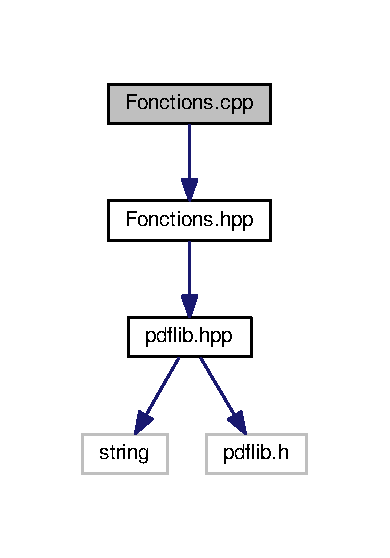
\includegraphics[width=187pt]{Fonctions_8cpp__incl}
\end{center}
\end{figure}

\hypertarget{Fonctions_8hpp}{\section{Fonctions.\+hpp File Reference}
\label{Fonctions_8hpp}\index{Fonctions.\+hpp@{Fonctions.\+hpp}}
}


\hyperlink{classFonctions}{Fonctions} permettant de générer des graphes au format pdf.  


{\ttfamily \#include \char`\"{}pdflib.\+hpp\char`\"{}}\\*
Include dependency graph for Fonctions.\+hpp\+:\nopagebreak
\begin{figure}[H]
\begin{center}
\leavevmode
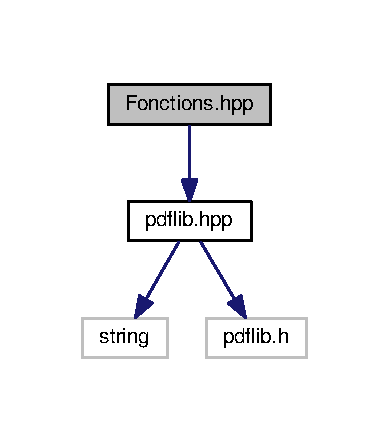
\includegraphics[width=187pt]{Fonctions_8hpp__incl}
\end{center}
\end{figure}
This graph shows which files directly or indirectly include this file\+:\nopagebreak
\begin{figure}[H]
\begin{center}
\leavevmode
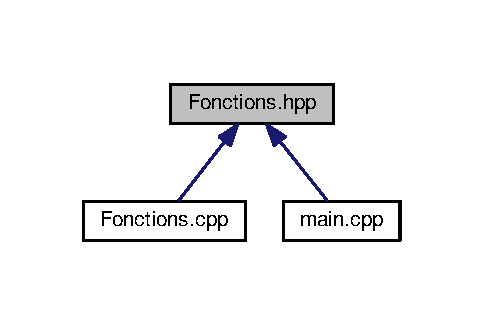
\includegraphics[width=232pt]{Fonctions_8hpp__dep__incl}
\end{center}
\end{figure}
\subsection*{Data Structures}
\begin{DoxyCompactItemize}
\item 
class \hyperlink{classFonctions}{Fonctions}
\begin{DoxyCompactList}\small\item\em classe intanciant un pdflib nous permettant d'executer des manipulations sur le pdf. \end{DoxyCompactList}\end{DoxyCompactItemize}
\subsection*{Macros}
\begin{DoxyCompactItemize}
\item 
\#define \hyperlink{Fonctions_8hpp_a3ff432d92eef82e8a8b12a29bd898a4a}{F\+O\+N\+C\+T\+I\+O\+N\+S\+\_\+\+H\+P\+P}
\end{DoxyCompactItemize}


\subsection{Detailed Description}
\hyperlink{classFonctions}{Fonctions} permettant de générer des graphes au format pdf. 

\begin{DoxyAuthor}{Author}
Dennis Bordet 
\end{DoxyAuthor}
\begin{DoxyVersion}{Version}
1.\+0 
\end{DoxyVersion}


\subsection{Macro Definition Documentation}
\hypertarget{Fonctions_8hpp_a3ff432d92eef82e8a8b12a29bd898a4a}{\index{Fonctions.\+hpp@{Fonctions.\+hpp}!F\+O\+N\+C\+T\+I\+O\+N\+S\+\_\+\+H\+P\+P@{F\+O\+N\+C\+T\+I\+O\+N\+S\+\_\+\+H\+P\+P}}
\index{F\+O\+N\+C\+T\+I\+O\+N\+S\+\_\+\+H\+P\+P@{F\+O\+N\+C\+T\+I\+O\+N\+S\+\_\+\+H\+P\+P}!Fonctions.\+hpp@{Fonctions.\+hpp}}
\subsubsection[{F\+O\+N\+C\+T\+I\+O\+N\+S\+\_\+\+H\+P\+P}]{\setlength{\rightskip}{0pt plus 5cm}\#define F\+O\+N\+C\+T\+I\+O\+N\+S\+\_\+\+H\+P\+P}}\label{Fonctions_8hpp_a3ff432d92eef82e8a8b12a29bd898a4a}

\hypertarget{main_8cpp}{\section{main.\+cpp File Reference}
\label{main_8cpp}\index{main.\+cpp@{main.\+cpp}}
}
{\ttfamily \#include $<$iostream$>$}\\*
{\ttfamily \#include \char`\"{}Fonctions.\+hpp\char`\"{}}\\*
Include dependency graph for main.\+cpp\+:\nopagebreak
\begin{figure}[H]
\begin{center}
\leavevmode
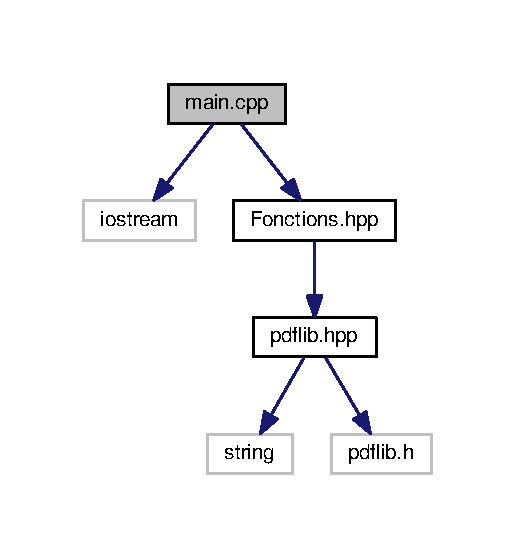
\includegraphics[width=247pt]{main_8cpp__incl}
\end{center}
\end{figure}
\subsection*{Functions}
\begin{DoxyCompactItemize}
\item 
int \hyperlink{main_8cpp_a840291bc02cba5474a4cb46a9b9566fe}{main} (void)
\end{DoxyCompactItemize}


\subsection{Function Documentation}
\hypertarget{main_8cpp_a840291bc02cba5474a4cb46a9b9566fe}{\index{main.\+cpp@{main.\+cpp}!main@{main}}
\index{main@{main}!main.\+cpp@{main.\+cpp}}
\subsubsection[{main}]{\setlength{\rightskip}{0pt plus 5cm}int main (
\begin{DoxyParamCaption}
\item[{void}]{}
\end{DoxyParamCaption}
)}}\label{main_8cpp_a840291bc02cba5474a4cb46a9b9566fe}

\hypertarget{pdflib_8cpp}{\section{pdflib.\+cpp File Reference}
\label{pdflib_8cpp}\index{pdflib.\+cpp@{pdflib.\+cpp}}
}
{\ttfamily \#include \char`\"{}pdflib.\+hpp\char`\"{}}\\*
Include dependency graph for pdflib.\+cpp\+:\nopagebreak
\begin{figure}[H]
\begin{center}
\leavevmode
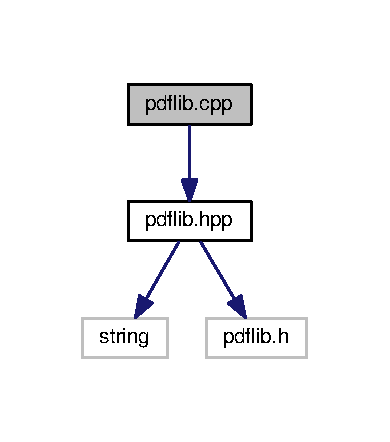
\includegraphics[width=187pt]{pdflib_8cpp__incl}
\end{center}
\end{figure}
\subsection*{Macros}
\begin{DoxyCompactItemize}
\item 
\#define \hyperlink{pdflib_8cpp_ac0471e02698206df72c7505ebaefcc1d}{C\+H\+A\+R}(s)~(s).c\+\_\+str()
\item 
\#define \hyperlink{pdflib_8cpp_af6116628d7f61b29fef302c9f32cc52f}{L\+E\+N}(s)~((int) (s).size())
\item 
\#define \hyperlink{pdflib_8cpp_aaa02a18eb619b1668268bf650a5c9aae}{P\+D\+F\+C\+P\+P\+\_\+\+T\+R\+Y}~P\+D\+F\+\_\+\+T\+R\+Y(p)
\item 
\#define \hyperlink{pdflib_8cpp_a633710be0517e8b60a87a356df4720c9}{P\+D\+F\+C\+P\+P\+\_\+\+C\+A\+T\+C\+H}
\end{DoxyCompactItemize}


\subsection{Macro Definition Documentation}
\hypertarget{pdflib_8cpp_ac0471e02698206df72c7505ebaefcc1d}{\index{pdflib.\+cpp@{pdflib.\+cpp}!C\+H\+A\+R@{C\+H\+A\+R}}
\index{C\+H\+A\+R@{C\+H\+A\+R}!pdflib.\+cpp@{pdflib.\+cpp}}
\subsubsection[{C\+H\+A\+R}]{\setlength{\rightskip}{0pt plus 5cm}\#define C\+H\+A\+R(
\begin{DoxyParamCaption}
\item[{}]{s}
\end{DoxyParamCaption}
)~(s).c\+\_\+str()}}\label{pdflib_8cpp_ac0471e02698206df72c7505ebaefcc1d}
\hypertarget{pdflib_8cpp_af6116628d7f61b29fef302c9f32cc52f}{\index{pdflib.\+cpp@{pdflib.\+cpp}!L\+E\+N@{L\+E\+N}}
\index{L\+E\+N@{L\+E\+N}!pdflib.\+cpp@{pdflib.\+cpp}}
\subsubsection[{L\+E\+N}]{\setlength{\rightskip}{0pt plus 5cm}\#define L\+E\+N(
\begin{DoxyParamCaption}
\item[{}]{s}
\end{DoxyParamCaption}
)~((int) (s).size())}}\label{pdflib_8cpp_af6116628d7f61b29fef302c9f32cc52f}
\hypertarget{pdflib_8cpp_a633710be0517e8b60a87a356df4720c9}{\index{pdflib.\+cpp@{pdflib.\+cpp}!P\+D\+F\+C\+P\+P\+\_\+\+C\+A\+T\+C\+H@{P\+D\+F\+C\+P\+P\+\_\+\+C\+A\+T\+C\+H}}
\index{P\+D\+F\+C\+P\+P\+\_\+\+C\+A\+T\+C\+H@{P\+D\+F\+C\+P\+P\+\_\+\+C\+A\+T\+C\+H}!pdflib.\+cpp@{pdflib.\+cpp}}
\subsubsection[{P\+D\+F\+C\+P\+P\+\_\+\+C\+A\+T\+C\+H}]{\setlength{\rightskip}{0pt plus 5cm}\#define P\+D\+F\+C\+P\+P\+\_\+\+C\+A\+T\+C\+H}}\label{pdflib_8cpp_a633710be0517e8b60a87a356df4720c9}
{\bfseries Value\+:}
\begin{DoxyCode}
PDF\_CATCH(p) \{\(\backslash\)
    throw Exception(PDF\_get\_errmsg(p), PDF\_get\_errnum(p),\(\backslash\)
                PDF\_get\_apiname(p), PDF\_get\_opaque(p));\(\backslash\)
\}
\end{DoxyCode}
\hypertarget{pdflib_8cpp_aaa02a18eb619b1668268bf650a5c9aae}{\index{pdflib.\+cpp@{pdflib.\+cpp}!P\+D\+F\+C\+P\+P\+\_\+\+T\+R\+Y@{P\+D\+F\+C\+P\+P\+\_\+\+T\+R\+Y}}
\index{P\+D\+F\+C\+P\+P\+\_\+\+T\+R\+Y@{P\+D\+F\+C\+P\+P\+\_\+\+T\+R\+Y}!pdflib.\+cpp@{pdflib.\+cpp}}
\subsubsection[{P\+D\+F\+C\+P\+P\+\_\+\+T\+R\+Y}]{\setlength{\rightskip}{0pt plus 5cm}\#define P\+D\+F\+C\+P\+P\+\_\+\+T\+R\+Y~P\+D\+F\+\_\+\+T\+R\+Y(p)}}\label{pdflib_8cpp_aaa02a18eb619b1668268bf650a5c9aae}

\hypertarget{pdflib_8hpp}{\section{pdflib.\+hpp File Reference}
\label{pdflib_8hpp}\index{pdflib.\+hpp@{pdflib.\+hpp}}
}
{\ttfamily \#include $<$string$>$}\\*
{\ttfamily \#include \char`\"{}pdflib.\+h\char`\"{}}\\*
Include dependency graph for pdflib.\+hpp\+:\nopagebreak
\begin{figure}[H]
\begin{center}
\leavevmode
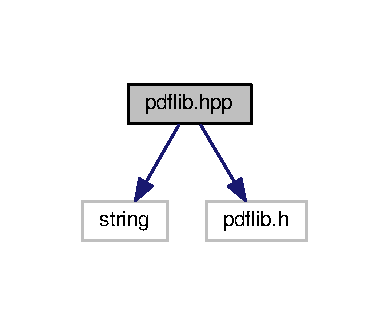
\includegraphics[width=187pt]{pdflib_8hpp__incl}
\end{center}
\end{figure}
This graph shows which files directly or indirectly include this file\+:\nopagebreak
\begin{figure}[H]
\begin{center}
\leavevmode
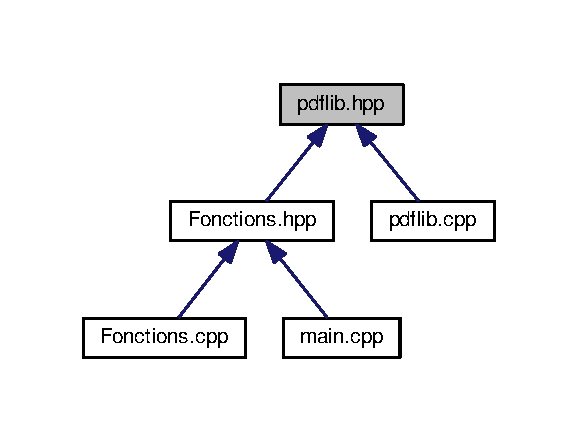
\includegraphics[width=277pt]{pdflib_8hpp__dep__incl}
\end{center}
\end{figure}
\subsection*{Data Structures}
\begin{DoxyCompactItemize}
\item 
class \hyperlink{classPDFlib}{P\+D\+Flib}
\item 
class \hyperlink{classPDFlib_1_1Exception}{P\+D\+Flib\+::\+Exception}
\end{DoxyCompactItemize}

%--- End generated contents ---

% Index
\newpage
\phantomsection
\addcontentsline{toc}{chapter}{Index}
\printindex

\end{document}
